\documentclass[
  a4paper,            % DIN A4
  DIV=10,             % Schriftgröße und Satzspiegel
  oneside,            % einseitiger Druck
  BCOR=5mm,           % Bindungskorrektur
  parskip=half,       % Halber Abstand zwischen Absätzen
  numbers=noenddot,   % Kein Punkt hinter Kapitelnummern
  bibtotoc,           % Literaturverzeichnis im Inhaltsverzeichnis
  listof=totoc,       % Abbildungs- und Tabellenverzeichnis im Inhaltsverzeichnis
  table
]{scrreprt}
\usepackage{../style/thesisstyle}
\usepackage{lipsum}
\usepackage{gensymb}
\usepackage{upgreek}
\usepackage{times}
\usepackage{amssymb}
\usepackage{hyperref}
\usepackage{xcolor}
% inline code highlighting
\newcommand{\code}[1]{\texttt{#1}}

\makeglossaries           % create all glossary entries (remember: run makeglossaries manually)
\loadglsentries{thesisglossaries.tex}  % load acronym, symbol and glossary entries

\sisetup{locale = DE}     % siunitx locale setup
%\DeclareSIUnit \fps{fps}  % a custom unit (usage: \SI{24}{\fps})

\begin{document}
% !TEX root = ../thesis.tex
%
% configurations
%

% English Language support
% -> uncomment if needed
% Beta!
%\fullenglish{yes}
\fullenglish{no}

% text field
%-> replace supervisor names with correct ones
\firstSupervisor{Prof. Dr. Philipp Jenke}
\secondSupervisor{Prof. Dr. Peer Stelldinger}

% text field
%-> replace title with your thesis title
\thesisTitle{Beispiel-basierte inverse prozedurale Generierung für zweidimensionale Szenen}
\thesisTitleEN{Example-based inverse procedural generation for two-dimensional scenes}

% text field
%-> replace the key words with your own key words
\keywordsDE{TODO SCHLÜSSELWÖRTER}
\keywordsEN{TODO KEYWORDS}

% text field
%-> replace the text with a description of the thesis
\abstractDE{TODO ZUSAMMENFASSUNG}
\abstractEN{TODO ABSTRACT}

% text field
%-> replace john with your name
\thesisAuthor{Benjamin Schröder}

% text field
%-> enter the submission date
\submissionDate{11. Juli 2024}

% switch - uncomment only one
%-> uncomment NDA or public
%\NDA{yes}
\NDA{no}

% switch - uncomment only one
%-> uncomment old standard cover or cover Corporate Design 2017
\Cover{CD2017}
%\Cover{CD2017NoLogo}
%\Cover{Std2018}
%\Cover{Std2018_green} 			% with green bar

% switch - uncomment only one
%-> uncomment to show list of figures or not
\ListOfFigures{yes}
%\ListOfFigures{no}

% switch - uncomment only one
%-> uncomment to show list of tables or not
\ListOfTables{yes}
%\ListOfTables{no}

% switch - uncomment only one
%-> uncomment to show list of accronyms or not
\ListOfAccronyms{yes}
%\ListOfAccronyms{no}

% switch - uncomment only one
%-> uncomment to show list of symbols or not
\ListOfSymbols{yes}
%\ListOfSymbols{no}

% switch - uncomment only one
%-> uncomment to show list of glossary entries or not
\Glossary{yes}
%\Glossary{no}

% switch - uncomment only one
%-> uncomment the study course you are in
%\studycourse{ITS}
%\studycourse{TI}
\studycourse{AI}
%\studycourse{WI}
%\studycourse{EI}
%\studycourse{REE}
%\studycourse{BMP}		
%\studycourse{BMP-hp}	 % Internship Report in M&P
%\studycourse{BMT}
%\studycourse{BMT-st}    % Study / home assignment in BMT
%\studycourse{BMT-hp}    % Internship Report in BMT
%\studycourse{MI}
%\studycourse{MIK}
%\studycourse{MA}

\def\imgHeight{100pt}
\def\imgWidth{420pt}
    % load all settings

\hyphenation{Ba-che-lor-the-sis Mas-ter-the-sis}

% Cover page here, no page number
\ICoverPage

% PDF Metadata
% !TEX root = ../thesis.tex
%
% PDF Metadata integration
% @author Thomas Lehmann
%

% PDF Metadata
\hypersetup{
pdftitle={\IthesisTitle},
pdfauthor={\IthesisAuthor},
pdfkeywords={\IkeyWordsEN}
}

% Titlepage is page one even if the number is not shown.
\pagenumbering{roman}
% Title page here
% !TEX root = ../thesis.tex
%
% title page
% @author Thomas Lehmann
% Hints for title page and page numbering: https://en.wikipedia.org/wiki/Title_page
%
\title{\IthesisTitle}   % set latex default title to be used by hyperref in pdf
\author{\IthesisAuthor} % set latex default author to be used by hyperref in pdf

\newpage
\thispagestyle{empty}
{\fontfamily{phv}\selectfont
  \hfuzz=20pt       % suppress warnings due to extension onto page margins

  % Author of thesis
  \vspace*{1cm}
  \begin{minipage}[b]{\textwidth}
    \fontsize{14pt}{20pt}
    \selectfont
    \begin{center}
      \IthesisAuthor
    \end{center}
  \end{minipage}

  % Title of thesis
  \vspace{1.5cm}
  \begin{minipage}[b][0cm][t]{\textwidth}
    \fontsize{18pt}{20pt}
    \selectfont
    \begin{center}
      \IthesisTitle
    \end{center}
  \end{minipage}

  % Important information
  \begin{textblock*}{\textwidth}(40mm,210mm)
    \begin{minipage}[b]{\textwidth}
      \hbadness=10001    % suppress underfull warning due to short text
      \fontfamily{cmr}\selectfont
      \fontsize{12pt}{14pt}
      \selectfont
      \ifdefined\ILanguageEN
        \IthesisKindEN ~submitted for examination in \IthesisExaminationEN \\
        in the study course \textit{\IstudyCourseName} \\
        at the \IthesisDepartmentFullEN \\
        at the \IthesisFacultyFullEN \\
        at University of Applied Science Hamburg\\

        Supervisor: \IfirstSv \\
        \ifdefined\IisTermPaper
          % left blank
        \else
          \ifdefined\IisInternshipReport
	  Supervised: \IsecondSv\\
          \else
        Supervisor: \IsecondSv \\
          \fi\fi
        
        Submitted on: \ISubDate \\
      \else
      	\ifdefined\IisInternshipReport
        \IthesisKindDE ~eingereicht im Rahmen des \IthesisExaminationDE \\	
	\else
        \IthesisKindDE ~eingereicht im Rahmen der \IthesisExaminationDE \\
        \fi
	im Studiengang \textit{\IstudyCourseName} \\
        am \IthesisDepartmentFull \\
        der \IthesisFacultyFull \\
        der Hochschule für Angewandte Wissenschaften Hamburg\\

        Betreuender Prüfer: \IfirstSv \\
        \ifdefined\IisTermPaper
          % left blank
        \else
          \ifdefined\IisInternshipReport
        betriebliche Betreuung: \IsecondSv \\							
	  \else
        Zweitgutachter: \IsecondSv \\
        \fi\fi

        Eingereicht am: \ISubDate \\
      \fi
    \end{minipage}
  \end{textblock*}
}


% Abstract page here
% !TEX root = ../thesis.tex
%
% abstract page
% @author Thomas Lehmann
%
\newpage
\thispagestyle{plain}
\clearpage
\hfuzz=12pt       % suppress warnings due to extenstion onto page margins

\textbf{\IthesisAuthor}

\vspace{0.3cm}
\textbf{Thema der Arbeit}

\IthesisTitle

\vspace{0.3cm}
\textbf{Stichworte}

\IkeyWordsDE

\vspace{0.3cm}
\textbf{Kurzzusammenfassung}

\begin{minipage}{\textwidth}
\IabstractDE
\end{minipage}

\vspace{1.0cm}
\textbf{\IthesisAuthor}

\vspace{0.3cm}
\textbf{Title of Thesis}

\IthesisTitleEN

\vspace{0.3cm}
\textbf{Keywords}

\begin{minipage}{\textwidth}
\IkeyWordsEN
\end{minipage}

\vspace{0.3cm}
\textbf{Abstract}

\IabstractEN


% Table of contents here
\tableofcontents

% List of figures here
\IListOfFigures

% List of tables here
\IListOfTables

% List of accronyms here
\IListOfAccronyms

% List of symbols here
\IListOfSymbols

% Uncomment if list of source code is needed (rarely).
%\lstlistoflistings  % requires package listings, needs to uncommenting of usepackage

% path to the chapters folder is set to find the images used there
\graphicspath{ {./chapters/} }

% Chapters
\clearpage
\pagenumbering{arabic}
% @author Benjamin Schröder
%
\chapter{Einleitung}

\section{Motivation}
% In diesem Abschnitt wird erklärt, wieso die prozedurale Generierung überhaupt so ein wichtiges Thema ist.
% Es wird geklärt, wer davon Gebrauch macht, und wieso es für den entsprechenden Anwender Sinn macht. Dazu zählt
% zum Einen das Einsparen von Ressourcen, aber auch das Umsetzen von Spielkonzepten, die durch die hier vorgestellten
% Verfahren erst möglich werden.
Die Erstellung von fiktiven Welten spielt eine große Rolle in vielen Videospielen, Filmen, Virtual Reality Umgebungen
und weiteren Bereichen der Simulation. Hierfür wird eine Vielzahl an verschiedenen Objekten und Strukturen benötigt, um
ein nicht-repetitives und immersives Erlebnis für den Endnutzer zu schaffen. All dies manuell anzufertigen, stellt vor
allem kleinere Indie-Entwicklerstudios vor eine große Herausforderung und kann die Entwicklungszeit signifikant in die
Länge ziehen. Aber auch in größeren Teams mit einer Vielzahl von Designern nimmt die Erstellung von realistischen Welten einen
Großteil der Entwicklungszeit in Anspruch und kann viele Monate dauern. \cite{10_freiknecht} Hier kann an einigen Stellen
nachgeholfen werden, indem man das Erstellen von Inhalten automatisiert. Entsprechende Prozesse lassen sich dem Bereich
der prozeduralen Generierung zuordnen.

Mithilfe von verschiedensten Verfahren können so z.B. einzelne Dungeons oder sogar ganze Welten und darin enthaltene Gebilde
automatisch erzeugt werden. Diese können eine Grundstruktur für ein komplexeres Design bilden, bei dem die Entwickler dann nur noch
kleinere Details per Hand abändern oder hinzufügen müssen. \cite{10_freiknecht} Andererseits existieren auch viele Videospiele,
wie z.B. Minecraft\footnote{\url{https://www.minecraft.net/} [Letzter Zugriff am 01.07.2024]} oder Terraria\footnote{
\url{https://terraria.org/} [Letzter Zugriff am 01.07.2024]}, die auf prozeduraler
Generierung aufbauen, um ihr Spielkonzept umzusetzen. Konkret wird einem neuen Spieler hier eine komplett neue und einzigartige,
aber dennoch logisch zusammenhängende Welt generiert; dies vollautomatisch und ohne zusätzlichen Aufwand für die Entwickler. Jeder
Spieler bekommt so eine einzigartie Erfahrung geboten und kann das Spiel außerdem gewissermaßen unbegrenzt oft durchspielen, ohne
dass es zu repetitiv wird. So etwas wäre ohne Automatisierung gar nicht erst umsetzbar.

\section{Problemstellung}
% Hier wird dann darauf aufmerksam gemacht, dass es bei diesen Verfahren viele Limitationen gibt. Bei vielen Verfahren
% ist es nötig, manuell Regeln für den Algorithmus zu erstellen, sodass dieser überhaupt arbeiten kann. Dies setzt wiederum
% einiges an Kenntnissen voraus und ist somit nicht für jeden zugänglich. Außerdem werden weitere Probleme aufgezeigt.

% Alte Formulierung:
% Es gibt viele bekannte Verfahren, welche solche Ergebnisse unter der Verwendung von u.a. zellulären Automaten, generativen
% Grammatiken oder Constraint-basierten Graphen erzielen können. \cite{5_van_der_linden_et_al} Ein Großteil dieser Verfahren erfordert jedoch
% menschliches Eingreifen in einigen der Teilschritte. So z.B. muss beim Verwenden einer generativen Grammatik meist bereits eine Menge
% an Produktionsregeln durch einen Menschen vorgegeben werden, bevor die automatische Generierung überhaupt beginnen kann. Das Erstellen
% solcher Regeln ist mit viel Arbeit und Trial-and-Error verbunden und kann ohne ein ausgeprägtes Verständnis des angewandten Verfahrens
% sehr schwierig werden. Dadurch kommt es für viele Designer letztendlich doch nicht in Frage. Auch gibt es Szenarien, in denen die Generierung
% von Inhalten durch den Endnutzer beeinflusst werden kann, so z.B. in Spielen, in denen der Spieler dynamisch mit dem Terrain und anderen
% Strukturen interagieren kann. In einem solchen Fall kann der Entwickler keinen direkten Einfluss auf den Generierungsprozess nehmen und alles
% muss voll automatisiert sein. \cite{14_carli_et_al} Hier setzt diese Arbeit an und untersucht Möglichkeiten zur vollständigen Automatisierung
% solcher Verfahren.

Es gibt viele bekannte Verfahren, welche solche Ergebnisse unter der Verwendung von u.a. generativen
Grammatiken oder Constraint-basierten Graphen erzielen können. \cite{5_van_der_linden_et_al} Ein Großteil dieser Verfahren erfordert jedoch
menschliches Eingreifen in einige der Teilschritte, was in einigen Szenarien zu einem Problem werden kann. Hängt die Generierung von
Inhalten eines Produkts z.B. von Entscheidungen des Endnutzers ab (z.B. in Spielen, in denen der Spieler dynamisch mit
dem Terrain und anderen Strukturen interagiert), so kann der Entwickler keinen direkten Einfluss auf den Generierungsprozess
nehmen und alles muss voll automatisiert sein. \cite{14_carli_et_al} Auch in Projekten, in denen dies nicht der Fall ist und der gesamte Inhalt
im Voraus erstellt wird, kann das Voraussetzen von menschlicher Intervenierung als Teil des Prozesses zu einem Problem werden.
Ein Beispiel hierfür wären Verfahren, die eine generative Grammatik nutzen und voraussetzen, dass dafür zunächst eine Menge an Regeln
durch einen Menschen vorgegeben wird, bevor die automatische Generierung überhaupt beginnen kann (z.B. \cite{33_adams}\footnote{
\url{https://citeseerx.ist.psu.edu/document?repid=rep1&type=pdf&doi=25020f8d955aee07b7dd49a3ec23b1f2a8cf1d06} [Letzter Zugriff am 01.07.2024]}).
Das Erstellen solcher Regeln ist mit viel Arbeit verbunden und kann ohne ein ausgeprägtes Verständnis des angewandten Verfahrens sehr
schwierig werden, wodurch der Einsatz eines solchen Verfahrens für viele Designer letztendlich doch nicht in Frage kommen wird. Hier
setzt diese Arbeit an und untersucht Möglichkeiten zur Automatisierung des Erstellens solcher Regeln.

\section{Ziele und Vorgehen}
% Aus den aufgezeigten Problemen ergibt sich nun der Sinn dieser Arbeit. Inverse Verfahren beheben die oben genannten Probleme
% und sollen deswegen genauer untersucht werden. Es werden verschiedene Verfahren analysiert und miteinander verglichen.
% Anschließend wird ein entsprechendes und vielversprechendes Verfahren im Detail untersucht, theoretisch erläutert und
% dann prototypisch implementiert.
Spezifisch soll versucht werden, Muster in Beispielstrukturen zu identifizieren. Aus diesen Mustern sollen dann Regeln zum Zusammensetzen
von Strukturen mit ähnlichen Eigenschaften abgeleitet werden. Gelingt dies, so muss ein Designer lediglich ein einziges Beispielmodell erstellen und
kann damit eine kreative Vision vorgeben. Alle weiteren Schritte zum Ableiten von Variationen dieses Inputs laufen anschließend automatisch ab.
Dies nennen wir \textit{inverse} prozedurale Generierung,
da der Prozess mit einem soweit fertigen Modell beginnt und daraus dann die Regeln ableitet, statt wie in den klassischen Verfahren zuerst mit
der Erstellung der Regeln zu beginnen. Die Erstellung eines Beispielmodells erfordert zwar nach wie vor die Arbeit eines Designers, anschließend
ist aber kein menschliches Eingreifen mehr nötig und das eigentliche Verfahren läuft vollautomatisch ab.

Es gibt bereits verschiedene Verfahren, die einen solchen Ansatz verfolgen. Diese sind u.a. der Gitter-basierte Wave Function
Collapse Algorithmus von Maxim Gumin \cite{45_gumin} oder die nach Symmetrien suchende inverse prozedurale Modellierung von Bokeloh
et al. \cite{3_bokeloh_et_al}.

Im Rahmen dieser Arbeit werden entsprechende Verfahren grob analysiert, deren Probleme aufgezeigt und anschließend ein neuer Ansatz vorgestellt,
welcher die vorhandenen Probleme minimieren soll. Das Endergebnis der Arbeit soll dann sein, dass die Funktionsweise des neuen Konzepts
ausführlich und verständlich dargestellt, und dieses anschließend prototypisch implementiert wird. Wir begrenzen uns dabei auf die Generierung von
Strukturen im zweidimensionalen Raum. Der gleiche Ansatz kann auch auf den dreidimensionalen Raum erweitert werden, um so vielseitiger einsetzbar zu
sein, jedoch reicht die vereinfachte Betrachtung zum Darstellen aller fundamentalen Konzepte.
% @author Benjamin Schröder
%
% Quellen: 5, 9, 10, 14, 15, 16, 17, 18, 19, 24, 25
%
% 5:
%   - Definition von PCG
%   - Vorstellen von einigen Verfahren
%
% 9:
%   - Definition von PCG durch Abgrenzung von anderen Verfahren
%
% 10:
%   - Geschichte und Verwendung von PCG
%   - Vorstellen einiger Verfahren
%
% 14:
%   - Vorstellen einiger Verfahren
%   - Unterscheidung zwischen assisted/non-assisted
%
% 15: The Death of the Level Designer
%   - kurze Definition von PCG
%   - Übersicht zu verschiedenen Anwendungsmöglichkeiten von PCG
%
% 16: An Image Synthesizer
%   - Perlin Noise
%
% 17: A Survey of Procedural Noise Functions
%   - Verwendung von Noise für PCG
%
% 18: Improving Noise
%   - Verbesserung von Perlin Noise
%
% 19: Fractals and the Geometry of Nature
%   - Fraktale (Mandelbrot)
%
% 24: A Very Short History of Dynamic and Procedural Content Generation
%   - Geschichte von PCG
%
% 25: Procedural Content Generation for Games: A Survey
%   - Klassifikation verschiedener Arten von PCG
%
% Weitere Links:
%   - https://en.wikipedia.org/wiki/Procedural_generation
%   Perlin Noise:
%   - https://mzucker.github.io/html/perlin-noise-math-faq.html#whatsnoise
%   - https://adrianb.io/2014/08/09/perlinnoise.html
%   - https://mrl.cs.nyu.edu/~perlin/doc/oscar.html
%   Simplex Noise:
%   - https://thebookofshaders.com/11/?lan=de

\chapter{Stand der Technik}
Als Grundlage für das Verständnis des weiteren Inhalts dieser Arbeit machen wir zunächst einen kurzen Abstecher in den
Bereich der prozeduralen Generierung allgemein. Wir stellen klar, was unter diesem Begriff zu verstehen ist und widmen
uns außerdem kurz der zugrundeliegenden Geschichte. Dabei werden wir einige fundamentale Errungenschaften und Verfahren
betrachten, die den Weg zum aktuellen Forschungsstand geprägt haben.

\section{Prozedurale Generierung}
Prozedurale Generierung, oder auch \gls{ac:pcg}, beschreibt eine Menge von Verfahren zum algorithmischen Erstellen von
Inhalten (``Content''). Dabei handelt es sich meist um Inhalte in Form von Texturen oder verschiedenen Gebilden im Kontext
von Videospielen und anderen Simulationen, wie z.B. Landschaften, Flüsse, Straßennetze, Städte oder Höhlenstrukturen.
\cite{14_carli_et_al} Auch Musik kann durch solche Verfahren generiert werden. \cite{28_ramanto_maulidevi}

Diese Definition ist absichtlich etwas allgemeiner gehalten, da das Aufstellen einer spezifischeren Definition nicht
besonders trivial ist. Das Konzept von \gls{ac:pcg} wurde bereits aus vielen veschiedenen Blickwinkeln beleuchtet und
ist für verschiedene Personen von unterschiedlicher Bedeutung. So hat z.B. ein Game Designer eine etwas andere Perspektive
als ein Wissenschaftler, der sich lediglich in der Theorie mit der Thematik beschäftigt. \cite{9_togelius_et_al}
Verschiedene Definitionen unterscheiden sich in Bezug auf Zufälligkeit, die Bedeutung von ``Content'', oder darin, ob und
in welchem Umfang menschliche Intervenierung eine Rolle in einem Verfahren spielen darf. Smelik et al. definieren ``Content''
als jegliche Art von automatisch generierten Inhalten, welche anhand von einer begrenzten Menge an Nutzer-definierten
Parametern erzeugt werden können. \cite{26_smelik_et_al} Timothy Roden und Ian Parberry beschreiben entsprechende Verfahren zur
Erzeugung dieser Inhalte als \textit{Vermehrungsalgorithmen} (``amplification algorithms''), da diese eine kleinere Menge
von Inputparametern entgegennehmen und diese in eine größere Menge an Outputdaten transformieren. \cite{27_roden_parberry}
Togelius et al. \cite{9_togelius_et_al} versuchen den Bereich genauer abzugrenzen, indem sie anhand von Gegenbeispielen
aufzeigen, was \textit{nicht} als \gls{ac:pcg} bezeichnet werden sollte. So zählt für Togelius et al. z.B. das Erstellen von
Inhalten eines Videospiels mittels Level-Editor in keinem Fall als \gls{ac:pcg}, auch wenn dabei das Spiel indirekt durch z.B.
automatisches Hinzufügen oder Anpassen von Strukturen beeinflusst wird. Generell wird sich in der Arbeit
von Togelius et al. \cite{9_togelius_et_al} ausführlich mit dem Problem der Definition von \gls{ac:pcg} befasst, weshalb
dies hier nun nicht weiter thematisiert werden soll. Die oben genannte grobe Erklärung fasst die Kernaussage der verschiedenen
Definitionen weitesgehend zusammen und sollte für unsere Zwecke ausreichen.

\section{Klassische Verfahren}
Schauen wir uns nun an, welche Verfahren über die Jahre hin entwickelt worden sind, um zu verstehen,
wie wir zum momentanen Stand der Technik gekommen sind.

\subsection{PRNG}
Einer der ersten und simpelsten Ansätze für \gls{ac:pcg} beruht auf der Generation von Pseudozufallszahlen (``pseudo random number
generation (PRNG)''). \cite{25_hendrikx_et_al} Das ab 1982 entwickelte und 1984 veröffentlichte Weltall-Erkundungsspiel ``Elite''
benutzt einen solchen Ansatz, um Eigenschaften der dort zu erkundenen Planeten automatisch zu generieren. \cite{36_spufford}
Diese Idee enstand aufgrund der technischen Limitationen zur damaligen Zeit. Die Entwickler, David Braben und Ian Bell, wollten den Spielern
eine Vielzahl an verschiedenen Planeten zum Erkunden bereitstellen. Da in gängiger Hardware jedoch zu wenig Speicherplatz vorhanden war,
um alle geplanten Details für all diese Planeten unterzubringen, ist Braben und Bell die Idee gekommen, diese Details erst zur Laufzeit
generieren zu lassen und somit das vorliegende Problem zu umgehen. Die Idee für das verwendete Verfahren beruht auf der Fibonacci-Folge.
Diese beginnt mit den Ziffern \(0\)
und \(1\), woraus anschließend eine unendliche Folge an weiteren Zahlen generiert werden kann, indem die letzten beiden Zahlen der Folge
aufsummiert werden. So entsteht schließlich die Folge \(0, 1, 1, 2, 3, 5, 8, 13, 21, \dots\). Diese erzeugt natürlich keine zufällige Folge
an Zahlen, hat Braben und Bell jedoch auf eine Idee gebracht. Nutzt man statt den Ziffern \(0\) und \(1\) einfach ein beliebiges
Paar von Ziffern, so können viele verschiedene Sequenzen nach dem gleichen Prinzip generiert werden. Werden z.B. die Startziffern \(3\)
und \(6\) gewählt, so erhält man im nächsten Schritt eine \(9\). Wird die Sequenz dann weitergeführt, so wird eine \(15\) erhalten. Statt
die \(15\) jedoch unverändert als nächsten Element der Folge zu nutzen, kann auch lediglich die letzte Ziffer aus dieser extrahiert werden,
wodurch wir stattdessen eine \(5\) erhalten. Führt man die Sequenz nach diesem Prinzip weiter, erhält man eine Folge an Ziffern
(\(3, 6, 9, 5, 4, 9, 3, 2, 5, 7, 2, \dots\)), die zwar nicht zufällig sind, aber zufällig wirken (daher ``\textit{Pseudo}zufallszahlen'').
Diese Idee konnte anschließend fortgeführt und erweitert werden: statt nur Ziffern zu benutzen, können ebenfalls größere Zahlen genutzt werden.
Statt in jedem Schritt die letzten beiden Ziffern einfach aufzusummieren, können weitere Transformationen vorgenommen werden, um die nächste
Zahl der Sequenz zu bestimmen. Mittels dieses Vorgehens konnten Braben und Bell nun einen Algorithmus entwickeln, der quasi zufällige Zahlen
erzeugt. Anschließend wurden diese Zahlen genutzt, um verschiedenste Eigenschaften der generierten Sternensysteme zu bestimmen, wie z.B. dessen Größe,
dessen Position im Raum, die Anzahl an enthaltenen Planeten und die Preise von verschiedenen Items. Auch Namen und Beschreibungen von Planeten
oder Gegenständen konnten generiert werden, indem die generierten Zahlen zum Auswählen von Wörtern in einer vordefinierten Tabelle an Adjektiven
und Substantiven genutzt wurden. \cite{36_spufford}

\subsection{Fraktale}
Etwa im gleichen Zeitraum, in dem ``Elite'' entwickelt wurde, haben sich weitere fundamentale Ansätze im Bereich von \gls{ac:pcg} angebahnt,
welche auf die Erstellung einer anderen Art von prozeduralem ``Content'' abzielen: dem Erzeugen von natürlich wirkenden, organischen Strukturen.
1982 stellte Benoit Mandelbrot seine Erkenntnisse zum Zusammenhang zwischen dem Aufbau natürlicher Strukturen (wie z.B. Landschaften, Gebirge, \dots)
und der fraktalen Geometrie vor. \cite{19_mandelbrot}

\begin{figure}[t]
    \centering
    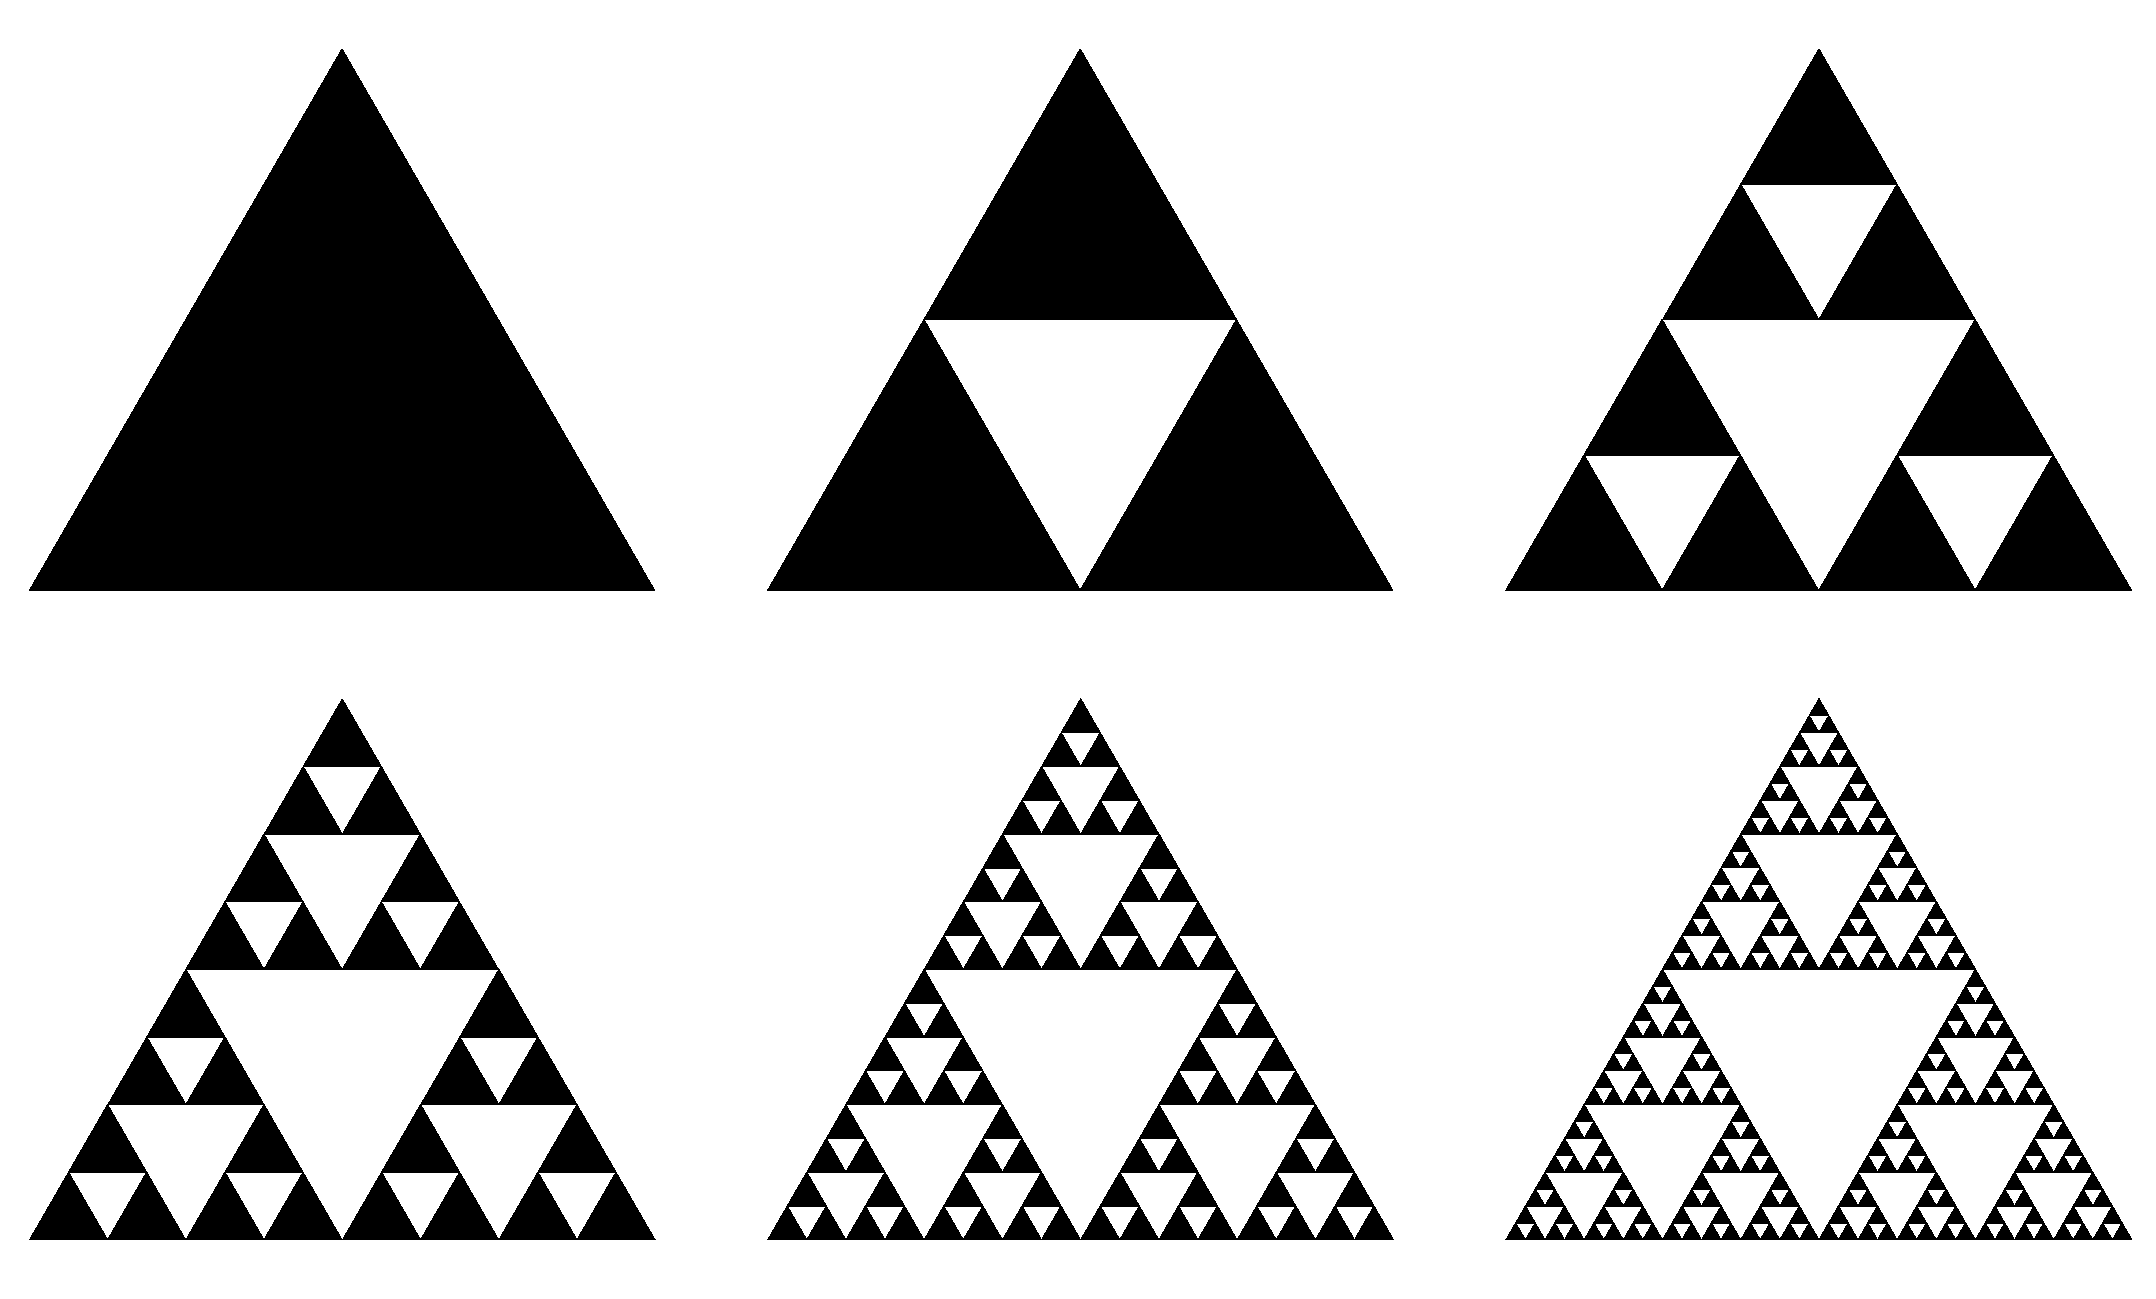
\includegraphics[width=(\imgWidth/2)]{images/sierpinski_triangle.pdf}
    \caption{Konstruktion eines Sierpinski Dreiecks.}
    \label{fig:sierpinski_triangle}
\end{figure}

Ein Fraktal ist ein geometrisches Objekt, das eine selbstähnliche Struktur aufweist. D.h. es sieht auf verschiedenen Skalen ähnlich oder identisch
aus. Das bedeutet, dass ein Teil des Fraktals eine verkleinerte Kopie des gesamten Fraktals ist. \cite{19_mandelbrot} Ein sehr bekanntes Beispiel
für eine solche Struktur ist das Sierpinski Dreieck. Dieses kann aus einem gleichseitigen Dreieck konstruiert werden,
indem man dieses mit drei kleineren gleichseitigen Dreiecken mit der halben Kantenlänge ersetzt, wobei in der Mitte eine Lücke entsteht. Ersetzt man
die neu enstandenen Dreieck immer wieder bis in's Unendliche nach dem gleichen Vorgehen, so ensteht das Sierpinski Dreieck. Die ersten paar Schritte
dieses Konstruktionsprozesses sind in Abbildung \ref{fig:sierpinski_triangle} zu erkennen. \cite{37_sierpinski} Eine simple Ersetzungsregel ermöglicht
hier das Bilden einer komplexen Struktur und kann technisch recht trivial mittels eines rekursiven Algorithmus umgesetzt werden. Fraktale lassen
sich häufig in der Natur wiederfinden, so z.B. in Schneeflocken, Küstenlinien, Wolken oder Pflanzen wie Brokkoli und Farnen, welche also algorithmisch
erzeugt werden können. \cite{19_mandelbrot}

\subsection{L-Systeme}
% ähnlich zu Fraktalen, ...

\subsection{Perlin Noise}
% gleiches Ziel wie Fraktal-Algorithmen
% diese jedoch sehr ineffzient, daher Verbesserung benötigt: Perlin Noise (Quelle 24: 2.2)
% Definition aus altem Grundlagenkapitel übernehmen und anpassen

\subsection{Zelluläre Automaten}



% l-systeme und zelluläre Automaten vllt zuerst vorstellen (chronologische Reihenfolge beibehalten)

\section{Inverse Verfahren}
% bis jetzt vorgestellte Verfahren hatten alles etwas gemeinsam: es wurden aufgrund von vordefinierten Regeln komplett neue Strukturen erzeugt
% -> inverse Ansätze gehen anders vor
\subsection{Model Synthesis}
% Merrell, Quellen 20-22
\subsection{Nutzen von partieller Symmetrie}
% Bokeloh et al., Quelle 3
\subsection{Wave Function Collapse}
\subsection{Inverses Ableiten einer Graph-Grammatik}
% Merrell, Quellen 1-2

% @author Benjamin Schröder
%
% Konzepte:
% - Splicing
% - Reduzierbarkeit (reducible graphs)
% - Irreducible Graphs (alle Graphen sind entweder reduzierbar oder unvollständig)

\chapter{Konzept}
Im Folgenden werden die theoretischen Konzepte hinter dem praktischen Teil der Arbeit betrachtet. Das implementierte Verfahren wird
Schritt für Schritt vorgestellt und im Detail erläutert. Die vorgestellten Konzepte beruhen auf den Erkenntnissen von Paul Merrell
in seiner Arbeit aus dem Jahr 2023 \cite{1_merrell}.

\section{Überblick}

\begin{figure}[t]
    \centering
    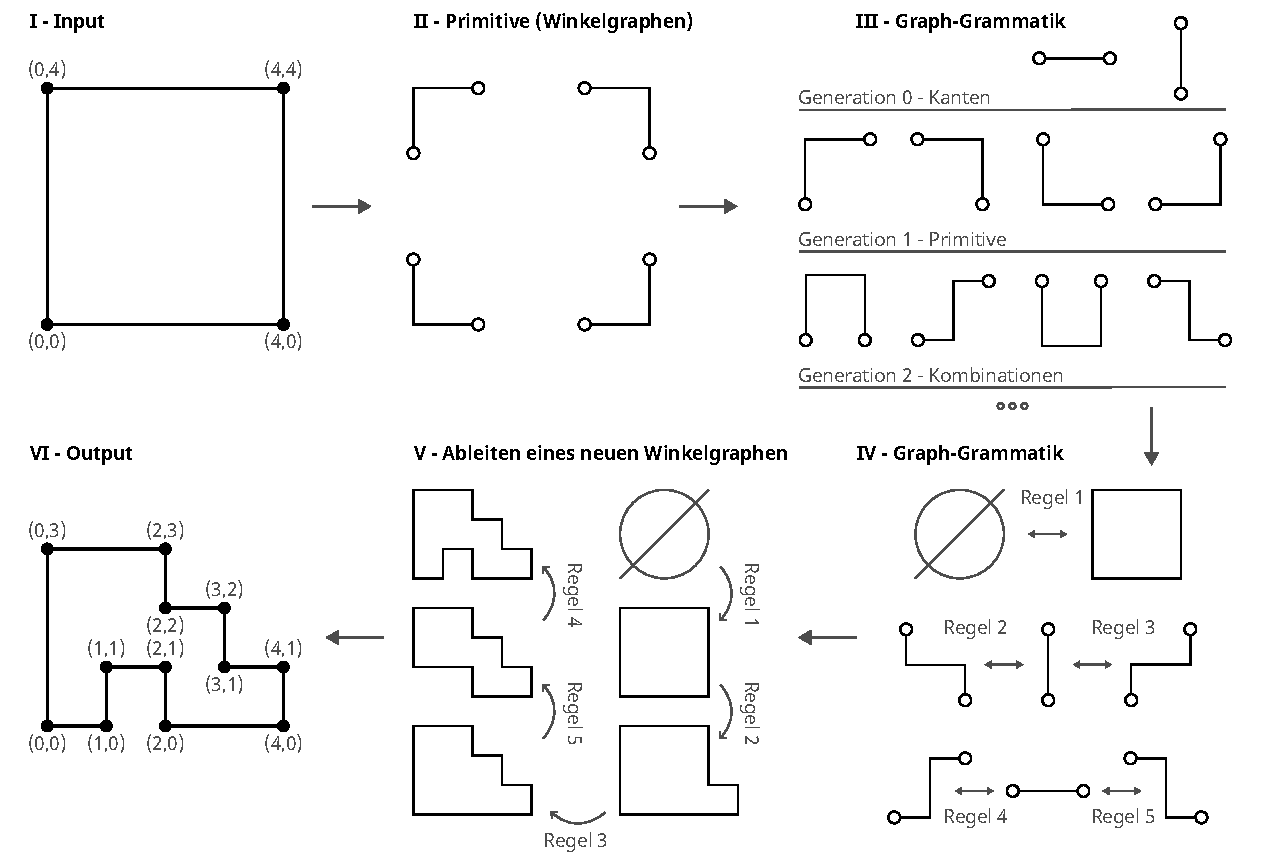
\includegraphics[width=\imgWidth]{images/overview.pdf}
    \caption{Überblick zum Ablauf des Verfahrens.}
    \label{fig:overview}
\end{figure}

Bevor es um die Einzelheiten und spezifischen Konzepte geht, wird zunächst ein grober Überblick zum Ablauf des umgesetzten
Verfahrens geliefert. Das Ganze beginnt mit einer polygonalen Inputstruktur, d.h. einem Gebilde bestehend aus einem oder mehreren Polygonen
(siehe Abbildung \ref{fig:overview}-I).
Diese Inputstruktur wird anschließend umgewandelt in einen Graphen, in welchem die konkrete Geometrie des Inputs keine Rolle
mehr spielt und sich auf die für das Verfahren wichtigen Eigenschaften des Inputs konzentriert werden kann.

Im nächsten Schritt wird der erstellte Graph nun in seine kleinstmöglichen Einzelteile zerlegt. Dazu werden alle Kanten in zwei Halbkanten
aufgeteilt. Das Ergebnis sind viele Teilgraphen, welche jeweils nur noch aus einem Knoten und einigen Halbkanten bestehen.
Einen solchen Teilgraphen nennen wir \textit{Primitiv}. Diese Primitive werden dann Schritt für Schritt in allen möglichen Kombinationen
zusammengeklebt, was zum Entstehen einer Hierarchie an immer komplexer werdenden Graphen führt (siehe Abbildungen \ref{fig:overview}-II und
\ref{fig:overview}-III).

Beim Aufbau der Hierarchie werden die neu entstehenden Graphen auf bestimmte
Eigenschaften überprüft, die es uns erlauben, daraus Regeln für eine Graph-Grammatik abzuleiten (siehe Abbildung \ref{fig:overview}-IV).
Das einfachste Beispiel hierfür sind
vollständige Graphen, also Graphen, die nur noch aus in sich geschlossenen Kreisen bestehen und keine Halbkanten mehr besitzen. Aus diesen lässt
sich eine sogennante Startregel ableiten, welche den leeren Graphen mit dem gefundenen vollständigen Graphen ersetzt. Das Finden von weiteren
Regeln ist deutlich komplizierter und wird später im Detail erläutert.

Sobald nun eine Menge von Regeln für die Graph-Grammatik gefunden wurde, kann man diese verwenden, um verschiedenste zum Inputgraphen
ähnliche Graphen abzuleiten. Dazu werden die gefundenen nach und nach zufällig angewendet, was man in Abbildung \ref{fig:overview}-V sehen kann.
Für einen solchen Graphen müssen dann nur noch konkrete Knotenpositionen und Kantenlängen bestimmt werden. (siehe Abbildung \ref{fig:overview}-VI).

\section{Grundlagen}
\subsection{Input}
Der Algorithmus kann mit beliebigen polygonalen Strukturen als Input arbeiten. Dies können einfache Rechtecke oder aber auch komplizierte Gebilde
aus verschiedenen Häusern oder ähnlichem sein. Wichtig ist lediglich, dass der Input als Sammlung von Polygonen beschrieben werden kann.

Ein Polygon ist eine geometrische Figur, die vollständig durch ein Tupel \(P\) von \(n\) verschiedenen Punkten beschrieben werden kann:
\[P = (P_1,P_2,\dots,P_n), P_i \in \mathbb{R}^2, 3 \leq i \leq n\]
Diese Punkte bezeichnen wir als \textit{Eckpunkte} des Polygons. Verbindet man zwei
aufeinanderfolgende Eckpunkte in Form einer Strecke \(\overline{P_i P_{i+1}}\) (für \(i = 1,\dots,n-1\)) bzw. \(\overline{P_n P_1}\) miteinander, so
erhält man eine \textit{Seite} des Polygons. All diese Seiten zusammen spannen das Polygon auf. Eine Beschränkung der Anzahl an Eckpunkten
nach oben gibt es dabei nicht, jedoch werden mindestens drei verschiedene Punkte für unsere Definition des Polygons vorausgesetzt. Mit weniger
als drei Punkten können lediglich Figuren ohne Fläche (Punkte, Linien) erzeugt werden, welche für uns nicht von Nutzen sind.
Ebenso sind Kreise oder andere Strukturen mit Rundungen nicht als Polygon darstellbar und können lediglich durch komplexe Polygone angenähert
werden. Der Input kann somit keine Rundungen enthalten.

Die einzelnen Polygone können außerdem mit Farben versehen werden, um verschiedene Arten von abgegrenzte Bereichen im Input zu markieren.

\subsection{Lokale Ähnlichkeit}
% Alte Formulierung:
% Ziel des Verfahrens ist es, Variationen des Inputs zu erzeugen. Dabei soll der Output eine gewisse Ähnlichkeit zum Input beibehalten. Global
% vorzugehen und die vollständigen Input- und Output-Strukturen miteinander zu vergleichen führt hierbei allerdings zu keinem brauchbaren
% Ergebnis. Der Output muss sich zumindest teilweise vom Input unterscheiden, ansonsten ist das Ergebnis nicht zu gebrauchen. Um Vergleiche
% auf einer kleineren Ebene vornehmen zu können, stellen wir hier das Konzept der \textit{lokalen Ähnlichkeit} vor. Das Verfahren gilt als
% erfolgreich, wenn die letztendlich erzeugten Output-Strukturen eine solche lokale Ähnlichkeit zum Input vorweisen können.

Das Ziel, das durch dieses Verfahren erreicht werden soll, ist es, Variationen des Inputs zu erzeugen. Die erzeugten
Output-Strukturen sollen dabei \textit{lokal ähnlich} zum gegebenen Input sein. Das Konzept der \textit{lokalen Ähnlichkeit} wird im Folgenden
vorgestellt. Das Verfahren gilt nur als erfolgreich, wenn diese zwischen Input und Output nachgewiesen werden kann.

Zwei Polygonstrukturen sind sich lokal ähnlich, wenn sich jeder Teil der einen Struktur zu einem Teil der anderen Struktur zuordnen lässt. Es
müssen sich also alle verschiedenen Arten von Kanten und alle Polygonfarben irgendwo in beiden Strukturen finden lassen. Ein verwandtes Konzept,
das zum Verständnis beitragen kann, ist das der \textit{r-Ähnlichkeit}, welche im Paper von Bokeloh et al. \cite{3_bokeloh_et_al} vorgestellt wurde.
Zwei Strukturen sind hier
\textit{r}-ähnlich, wenn wir für jeden Punkt innerhalb der einen Struktur einen Kreis mit Radius \textit{r} aufspannen können und sich der Inhalt
dieses Kreises (r-Nachbarschaft des Punktes) genauso in der anderen Struktur wiederfinden lässt. Ein Beispiel hierfür befindet sich in Abbildung
\ref{fig:rsimilarity}.

\begin{figure}[t]
    \centering
    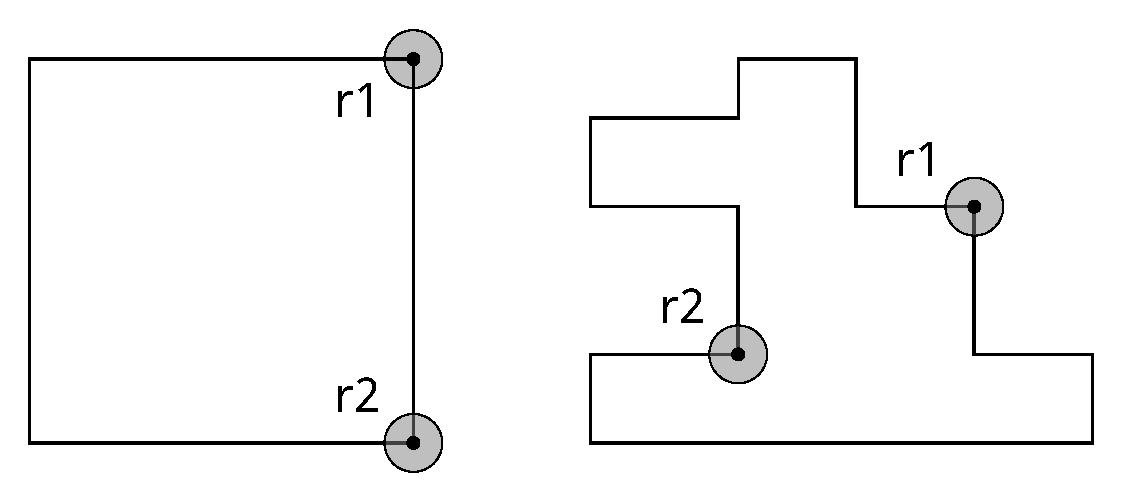
\includegraphics[height=\imgHeight]{images/rsimilarity.pdf}
    \caption{r-Ähnlichkeit.}
    \label{fig:rsimilarity}
\end{figure}

Die von uns verwendete lokale Ähnlichkeit funktioniert nach dem gleichen Konzept, mit der Ausnahme, dass der Radius so klein wie möglich gehalten
wird. Wir schauen uns also lediglich an, welche Kanten und Polygone direkt an einem Punkt anliegen, während uns die restliche Nachbarschaft
egal ist. So können die betrachteten Strukturen beliebig skaliert werden und trotzdem ihre lokale Ähnlichkeit zueinander bewahren, solang alle
Kantenwinkel dabei beibehalten werden.

\subsection{Der Winkelgraph}
Zur Verarbeitung des Inputs wird dieser in einen sogenannten Winkelgraphen umgewandelt, in welchem die spezifischen Positionen der Knoten
keine Rolle spielen. Stattdessen wird nur abgebildet, welche Knoten es überhaupt gibt, welche der Knoten durch Kanten miteinander verbunden
sind, und in welchem Winkel diese Kanten verlaufen.
Die Kanten im Graphen werden mit einem \textit{Kantenlabel} versehen, welches neben den Start- und Endknoten ebenfalls Informationen zum
daraus ableitbaren Tangentenwinkel, sowie zu den Farben der links und rechts anliegenden Polygone enthält. Ein Kantenlabel besitzt die Form
\(\tilde{k} = (l,r,\theta)\), wobei \(\tilde{k}\) die Bezeichnung der Kante, \(l\) und \(r\) die Farben der anliegenden Polygone, und
\(\theta\) der Tangentenwinkel der Kante sind.
Nach der Umwandlung des Inputs in einen Winkelgraphen ist dieser zunächst \textit{vollständig}, d.h. er besteht ausschließlich aus
geschlossenen Kreisen. In späteren Verarbeitungsschritten wird dieser allerdings in unvollständige Teilgraphen zerlegt, welche dann außerdem
\textit{Halbkanten} enthalten können. Im Gegensatz zu den vorher erwähnten Kanten sind diese gerichtet, können aber trotzdem durch ein
gleichartiges Kantenlabel beschrieben werden. In späteren Abschnitten wird noch etwas genauer auf die Relevanz von Halbkanten und deren
spezifische Notation eingegangen.

\subsubsection{Komplexität von Winkelgraphen}
Später müssen einige der erstellten Winkelgraphen miteinander verglichen werden. Dabei muss bestimmt werden können, welcher
von zwei Graphen komplexer bzw. simpler ist. Dies ist nicht schwierig, sollte jedoch einmal eindeutig definiert werden. Das ausschlaggebendste
Kriterium hierbei ist die Anzahl der Halbkanten der verglichenen Graphen. Ein Graph mit weniger
Halbkanten gilt direkt als simpler als ein Graph mit einer größeren Anzahl an Halbkanten. In vielen Fällen werden die verglichenen Graphen jedoch die gleiche Anzahl
an Halbkanten vorzuweisen haben. Hier wird die Graph-Hierarchie wichtig. Wurde ein Graph früher in die Hierarchie eingefügt, so gilt dieser als
simpler. Dies kann immer eindeutig bestimmt werden und es kommt zu keinen weiteren Konflikten.

\subsection{Planarität und der Graph Boundary String}
Damit die erzeugten Winkelgraphen später auch ohne Überschneidungen der Kanten dargestellt werden können, muss deren Planarität sichergestellt
werden. Die endgültig erzeugten vollständigen Winkelgraphen bestehen nur noch aus geschlossenen Kreisen. Diese können dann als Polygone
dargestellt werden, vorausgesetzt der jeweilige Kreis war planar.

Ein geschlossener Kreis ist planar, wenn wir uns beim Traversieren seiner Kanten exakt einmal um 360° gedreht haben. Wenn wir also iterativ
alle Kanten eines solchen Kreises gegen den Uhrzeigersinn betrachten, jeweils die Differenz der Winkel berechnen und diese Differenzen
aufsummieren, so erhalten wir einen Gesamtwinkel von 360°. Es kann allerdings auch vorkommen, dass wir beim Entlanglaufen eines Pfades um
einen geschlossenen Kreis herum einen Gesamtwinkel von mehr als 360° erhalten, so z.B. 720°. Ist dies der Fall, so muss sich der Pfad zwingend
selbst gekreuzt haben. Analog würde es bei der Darstellung der Kanten des entsprechenden Kreises mindestens eine unvermeidliche Überschneidung
geben. Somit wäre der Winkelgraph, der diesen Kreis enthalten hat nicht mehr planar, was in Abbildung \ref{fig:planarity} visuell verdeutlicht wird.

\begin{figure}[t]
    \centering
    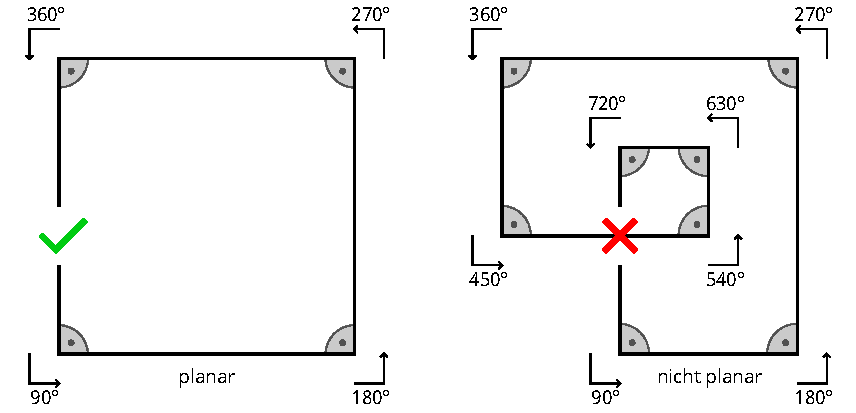
\includegraphics[width=(\imgWidth*3/4)]{images/planarity.pdf}
    \caption{Der Zusammenhang zwischen Drehwinkel und Planarität.}
    \label{fig:planarity}
\end{figure}

Zum Vorbeugen dieses Problems definieren wir hier das Konzept der \textit{Graph Boundary} und die dazugehörige Notation in Form vom
\textit{\gls{ac:gbs}}. Jeder Winkelgraph \(G\) besitzt eine solche Boundary \(\partial G\). Diese beschreibt einen Pfad außen um den entsprechenden
Winkelgraphen herum und enthält alle vorhandenen Halbkanten, sowie Informationen dazu, wie sich die Winkel entlang des Pfades ändern.
Der Pfad verläuft gegen den Uhrzeigersinn und hat keinen festen Startpunkt. Wichtig ist lediglich die relative Anordnung der enthaltenen
Elemente. Um dies abbilden zu können, muss sich der \gls{ac:gbs} nicht als Liste mit festem Start- und Endpunkt vorgestellt werden,
sondern als Kreis mit einer zusätzlichen Verbindung zwischen Anfang und Ende. Angenommen \(abc\wedge\) ist ein \gls{ac:gbs}, dann gilt
\(abc\wedge = bc\wedge a = c\wedge ab = \wedge abc\).

Um den aktuellen Drehwinkel in Relation zum Startpunkt des Pfades zu ermitteln, können wir uns jeweils die Kantenlabel der traversierten
Kanten anschauen und dort den Tangentenwinkel entnehmen. Dies wird allerdings problematisch, sobald sich der Pfad um mehr als
360° dreht, da die Tangentenwinkel bei 180° bzw. -180° umgebrochen werden. Berechnen wir den aktuellen Drehwinkel entlang der Graph Boundary mithilfe
dieser Tangentenwinkel, so können wir nie eine Differenz von über 360° erhalten. Haben wir uns vom Startpunkt aus z.B. tatsächlich um 400°
gedreht, so würde die hier berechnete Differenz lediglich \(400\degree - 360\degree = 40\degree\) betragen. Wir wissen also nie, ob wir uns
aktuell um den Winkel \(\theta\), \(\theta + 360\degree\), \(\theta + 720\degree\) oder noch mehr gedreht haben.
Dieses Problem lässt sich durch Einführung des Konzepts der \textit{positiven und negativen Drehungen} umgehen.

\textit{Positive Drehung \(\wedge\).} Dreht sich der Pfad aktuell gegen den Uhrzeigersinn wird der Winkel mit jeder gefundenen Kante größer. Stoßen wir
dabei allerdings auf den Schwellwert von 180°, so bricht der Winkel auf einmal in den negativen Bereich um. Diesen Umbruch bezeichnen wir als
positive Drehung. Folgen wir beim Entlanglaufen des Pfades dem Verlauf einer positiven Kanten und wechseln dann auf eine negativ verlaufende Kante, so
werden wir dabei in einigen Fällen diesen Schwellwert überschreiten. Falls dies geschieht, so fügen wir eine
positive Drehung in Form des Symbols \(\wedge\) in den \gls{ac:gbs} ein. Die Boundary eines planaren Winkelgraphen muss zwingend eine
solche positive Drehung enthalten.

\textit{Negative Drehung \(\vee\).} Die negative Drehung stellt das Gegenteil zur positiven Drehung dar. Dreht sich der Pfad aktuell im
Uhrzeigersinn, so nähern sich die gefunden Winkel nach und nach dem Schwellwert von -180°. Anschließend bricht der Winkel in den positiven Bereich
um, was wir als negative Drehung bezeichnen und mit dem Symbol \(\vee\) im \gls{ac:gbs} notieren.

\begin{figure}[t]
    \centering
    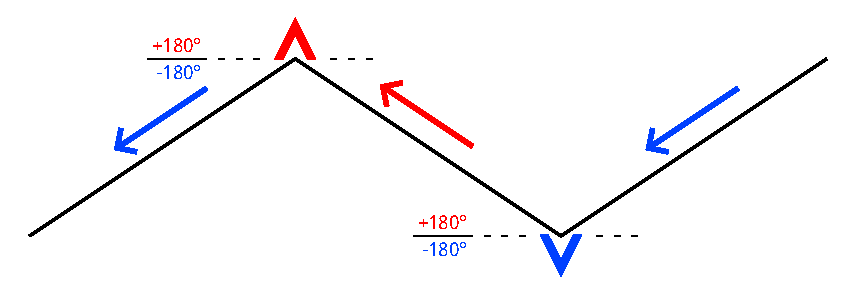
\includegraphics[width=(\imgWidth*3/4)]{images/turns.pdf}
    \caption{Positive und negative Drehungen.}
    \label{fig:turns}
\end{figure}

Die beiden in Abbildung \ref{fig:turns} zu sehenden Drehungen heben sich gegenseitig auf. Befinden sich eine positive und eine negative Drehung
nebeneinander im \gls{ac:gbs}, so können diese entfernt werden. Ebenfalls kann an jeder beliebigen Stelle ein ``\(\wedge\vee\)'' oder ein
``\(\vee\wedge\)'' eingefügt werden, ohne die Bedeutung des jeweiligen \gls{ac:gbs} zu verändern. Eine weitere Eigenschaft, die sich für den \gls{ac:gbs}
für alle planaren Winkelgraphen ergibt ist, dass sich darin immer genau eine positive Drehung mehr befinden muss, als es negative Drehungen gibt.
Dies liegt daran, dass sich der Pfad um einen planaren Graphen insgesamt exakt um 360° dreht und der Drehwinkel somit zumindest einmal irgendwo
den Schwellwert überschreiten muss. Da wir die Graph Boundary entgegen des Uhrzeigersinns ablaufen,
handelt es sich dabei um eine positive Drehung \(\wedge\).

\subsection{Teil-Operation}
Eine Kante \(\tilde{k}\) kann in zwei Halbkanten \(k\) und \(\overline{k}\) zerteilt werden. Im Gegensatz zu \(\tilde{k}\)
sind diese beiden Halbkanten gerichtet und zeigen in entgegengesetze Richtungen. Dabei zeigt \(k\) stets in positive Richtung und besitzt einen
positiven Tangentenwinkel \(\theta \in [0\degree,180\degree) \), während \(\overline{k}\) immer in negative Richtung zeigt und einen negativen
Tangentenwinkel \(\theta \in [-180\degree,0\degree) \) besitzt. Ein Tangentenwinkel von 0° zählt hier als positiv. Der entgegengesetze Winkel
von 180\degree\ gilt als negativ, da dieser ebenfalls als -180\degree\ interpretiert werden kann. Die Teil-Operation ermöglicht das Zerlegen vom
Input in seine Primitive.

\subsection{Klebe-Operation}
Zwei entgegengesetze Halbkanten \(k\) und \(\overline{k}\) können wieder zu einer vollständigen und ungerichteten Kante
\(\tilde{k}\) zusammengeklebt werden. Dies ermöglicht das Schließen von Kreisen innerhalb eines Graphen oder die Kombination von mehreren
kleineren Graphen, vorausgesetzt diese besitzen passende Halbkanten. Hier ist erneut der \gls{ac:gbs} von Relevanz, da aus diesem alle
möglichen Klebe-Operationen abgeleitet werden können, welche die Planarität der entstehenden Graphen bewahren. Grundlegend gibt es zwei
verschiedene Arten von Klebe-Operationen: Loop Gluing und Branch Gluing.

\textit{Loop Gluing} beschreibt das Zusammenkleben zweier Kanten innerhalb eines einzigen Graphen. Das Anwenden einer solchen Operation
führt zum Schließen eines Kreises innerhalb des Graphen. Ob ein Loop Gluing auf einen Graphen angewandt werden kann, lässt sich durch das
Vorhandensein eines der zwei Teilstrings ``\(a \overline{a}\)'' oder ``\(\overline{a}\vee a\wedge\)'' innerhalb des \gls{ac:gbs} ermitteln. Werden
die gefundenen Kanten dann zusammengeklebt, muss der \gls{ac:gbs} entsprechend angepasst werden. Für das Loop Gluing ist diese Anpassung
besonders einfach und es muss lediglich der gefundene Teilstring entfernt werden. Die entsprechenden String-Ersetzungen besitzen die Form:

\begin{center}
    \(a \overline{a} \longrightarrow \epsilon\) \ \ \ bzw. \ \ \ \(\overline{a}\vee a\wedge \longrightarrow \epsilon\) 
\end{center}

\textit{Branch Gluing} beschreibt das Zusammenkleben zweier Kanten von verschiedenen Graphen. Dies führt zur Vereinigung der beiden betroffenen
Graphen in einen neuen, größeren Graphen. Besitzt Graph \(G\) die Kante \(\overline{a}\) und Graph \(H\) die Kante \(a\), so kann ein Branch Gluing
durchgeführt werden. Hierbei gibt es wieder zwei Optionen:

\begin{center}
    \(\overline{a}G\) an \(a\): \(a \longrightarrow G \vee\) \ \ \ bzw. \ \ \ \(a H\) an \(\overline{a}\): \(\overline{a} \longrightarrow \vee H\)
\end{center}

Die Großbuchstaben G und H stehen hier jeweils für den Rest des \gls{ac:gbs} der beiden Graphen. Der \gls{ac:gbs} des neu enstandenen Graphen
stellt die Kombination der beiden kleineren \gls{ac:gbs} dar, allerdings ohne die zusammengeklebten Halbkanten und mit einer zusätzlichen
negativen Drehung.

\begin{figure}[t]
    \centering
    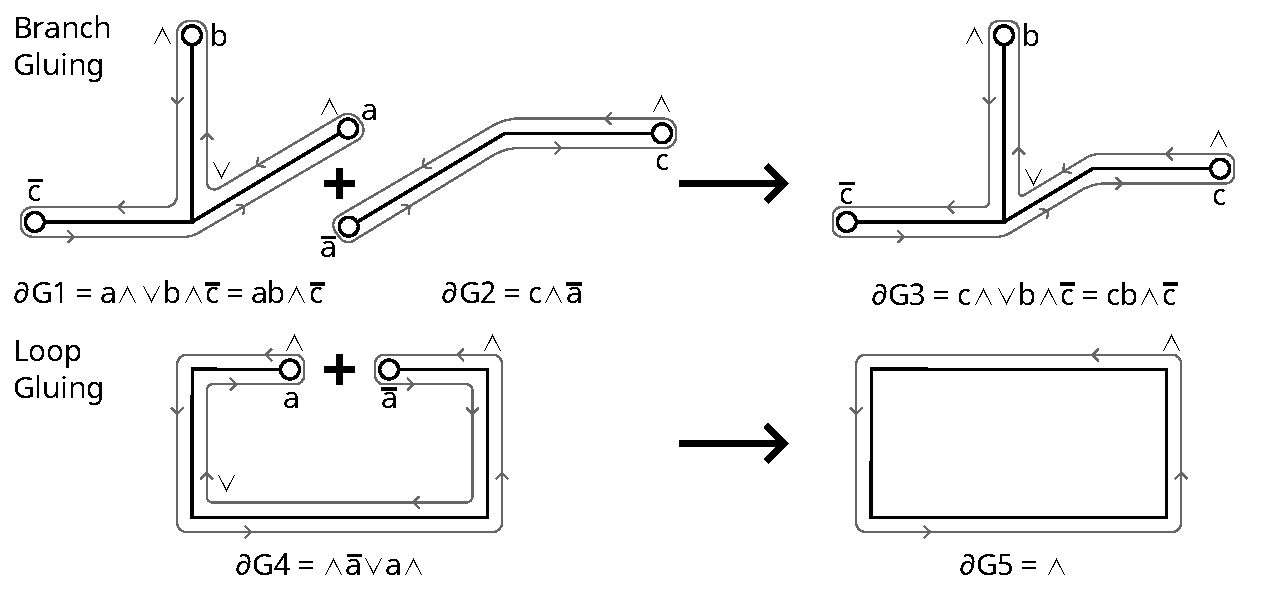
\includegraphics[width=(\imgWidth)]{images/gluing.pdf}
    \caption{Branch und Loop Gluing.}
    \label{fig:gluing}
\end{figure}

\section{Finden der Graph-Grammatik}
\subsection{Anpassen des Inputs}
% TODO: Anpassen oder Löschen
Bevor wir mit dem Verfahren beginnen können, muss der Input an bestimmte Anforderungen angepasst werden. Die übergebene Polygonstruktur
kann so nicht direkt verarbeitet werden und muss erst einmal in einen Winkelgraphen umgewandelt werden. Ohne diesen Schritt liegen uns keine
Informationen zu den Kantenwinkeln vor, welche ausschlaggebend für die weiteren Schritte sind. Hierzu werden zunächst einfach alle Knoten und
Kanten aus dem Input übernommen. Anschließend werden die Knotenpositionen genutzt, um den Verlauf der Kanten in Form eines Tangentenwinkels zu
ermitteln. Sobald dies geschehen ist, können die Knotenpositionen dann ignoriert werden, da lediglich die Ausrichtung der Kanten eine Rolle
für die weiteren Schritte spielt. Die restlichen Informationen zur Geometrie werden nicht benötigt und erst beim Erzeugen des finalen Outputs
wieder festgelegt.

\subsection{Finden der Primitive}
Ist nun der Winkelgraph ermittelt worden, können wir daraus die Primitive ableiten. Diese sind die fundamentalen Grundbausteine für das
gesamte Verfahren. Aus ihnen werden alle weiteren Strukturen abgeleitet, weshalb es besonders wichtig ist, diese korrekt und vollständig zu
ermitteln. Glücklicherweise wird dies durch die vorgestellte Teil-Operation recht trivial. Wenden wir diese auf jede Kante des gegebenen
Winkelgraphen an, so bleiben nur Teilgraphen übrig, welche nur aus einem einzelnen Knoten, sowie einigen Halbkanten bestehen. Diese Teilgraphen
sind dann auch schon die gesuchten Primitive. Hier können allerdings einige identische Teilgraphen entstehen, falls Teile des Input eine ähnliche
Struktur vorzuweisen hatten. Solche Duplikate sind nicht relevant für die weiteren Schritte und werden ignoriert.

\subsection{Aufbauen der Graph-Hierarchie}
Die vorgestellten Klebe-Operationen ermöglichen es uns, die gefundenen Primitive nach und nach zu komplexeren Graphen zusammenzusetzen.
Diese lassen sich in verschiedene Generationen einer Hierarchie einordnen. In Generation 0 befinden sich alle verschiedenartigen
Kanten, also alle Kanten mit einem einzigartigen Kantenlabel. In Generation 1 befinden sich alle gefundenen Primitive. Anschließend können daraus
die nachfolgenden Generationen automatisch generiert werden. Dazu wird durch alle Winkelgraphen der zuletzt generierten Generation iteriert
und alle durchführbaren Klebe-Operationen auf diese angewandt. Gibt es in einem der iterierten Graphen einen noch offenen Kreis, der aber
durch eine einfach Loop Gluing Operation geschlossen werden kann, so wird diese angwandt. Außerdem werden jeweils alle der gefundenen Primitive
betrachtet und ein Branch Gluing mit diesen ausgeführt, vorausgesetzt deren \gls{ac:gbs} lässt dies zu.
Wird durch eine dieser Operationen ein neuer Graph erzeugt, so gilt dieser als Kind des anderen Graphen. Jeder Graph wird
also neben der Einordnung in eine Generation außerdem in eine Eltern-Kind-Beziehung gebracht. Die Struktur der Hierarchie selbst ähnelt somit
fast der eines Baumes, allerdings kann ein und derselbe Kindsgraph durch verschiedene Elterngraphen erzeugt werden, wodurch wiederum Kreise
innerhalb der Hierarchie entstehen.

In der Theorie können alle Kombinationen an Primitiven erzeugt werden, wenn wir dieses Vorgehen bis in die Unendlichkeit weiterführen. Somit
würden garantiert alle zum Input lokal ähnlichen Winkelgraphen erzeugt werden und man könnte einfach jeden beliebigen vollständigen Graphen
aus der Hierarchie entnehmen, um jeden validen Output des Verfahrens erzeugen zu können. Praktisch gesehen ist dies natürlich leider nicht
umsetzbar, da uns weder unendlich viele Ressourcen noch Zeit zur Verfügung stehen. Um diesen Ansatz also praktisch zu machen, müssen einige
Anpassungen gemacht werden.

\subsection{Ableiten der Graph-Grammatik}
Statt zuerst eine ``vollständige'' Hierarchie zu erzeugen und aus
dieser dann weitere Schritte abzuleiten, wird die Hierarchie inkrementell erzeugt. Jedes Mal, wenn ein neuer Graph erstellt wird, überprüfen
wir diesen auf bestimmte Eigenschaften, die es uns erlauben daraus Regeln für eine Graph-Grammatik abzuleiten. Ein solche Regel ermöglicht es
uns bereits erzeugte Winkelgraphen zu reduzieren, was wiederum bedeutet, dass wir diese nicht mehr benötigen und aus der Hierarchie entfernen
können. Ein detaillierter Einblick zu der Theorie dahinter wird erst in den folgenden Unterkapiteln gegeben, jedoch ist es genau diese Eigenschaft,
die es uns ermöglicht, das Wachstum der Hierarchie einzugrenzen. Optimalerweise erreichen wir irgendwann einen Punkt, an dem alle bereits erzeugten
Graphen durch eine der Regeln reduziert werden konnten. In diesem Fall können wir garantieren, dass sich aus den Regeln alle vollständigen
und zum Inputgraphen lokal ähnlichen Winkelgraphen aus der erzeugten Grammatik ableiten lassen. Meistens werden wir allerdings auf
Szenarien stoßen, in denen die Anzahl der neuen Graphen schneller wächst, als wir andere Graphen entfernen können. Kommt dies vor, so muss das
Erstellen der Hierarchie irgendwann frühzeitig abgebrochen werden und die Graph-Grammatik ist eventuell nicht in der Lage, alle lokal ähnlichen
Graphen zu erzeugen. Trotzdem kann die Grammatik dann zum Ableiten einer Vielzahl von lokal ähnlichen Winkelgraphen genutzt werden.

\subsubsection{Graph-Grammatiken}
Bevor wir die Erzeugung dieser Datenstruktur genauer betrachten, soll erst einmal der Begriff der Graph-Grammatik klar definiert werden.
Eine Graph-Grammatik ist ein formales System, welches spezifisch auf die Erstellung und Manipulation von Graphen in einem mathematisch
präzisen Weg abzielt. Dazu wird eine Menge an Produktionsregeln definiert, welche verschiedene Operationen zum Ersetzen von Teilen
eines Graphen beschreiben. Eine solche Produktion besteht üblicherweise aus drei Bestandteilen: zwei Graphen \(M\) und \(T\) (``Mutter'' und
``Tochter''), sowie einem Einbettungsmechanismus \(E\). Diese Produktion kann nun auf jeden Graphen \(G\) angewandt werden, welcher \(M\)
als Teilgraphen enthält. Um die Produktion anzuwenden, wird \(M\) aus \(G\) entfernt und mit \(T\) ersetzt. Dabei wird \(E\) genutzt, um zu
definieren, wie genau \(T\) in \(G\) eingebettet werden kann. \cite{31_engelfriet_rozenberg}

Das Konzept der Graph-Grammatiken existiert bereits seit den frühen 70er Jahren und wurde mit dem Paper von Ehrig et al. \cite{7_ehrig_et_al}
zum ersten Mal formal definiert. Seitdem haben sich sehr viele verschiedene Herangehensweisen in diesem Kontext etabliert, was zu viel Verwirrung
führen kann. \cite{30_könig_et_al} Wir beschränken uns hier auf den ursprünglich präsentierten algebraischen bzw. Gluing-Ansatz von Ehrig 
et al. \cite{7_ehrig_et_al}. Innerhalb dieses Ansatzes haben sich zwei verschiedene Vorgehensweisen etabliert: der Single Pushout Ansatz und der
\gls{ac:dpo} Ansatz, wovon wir den letzteren verwenden. Der Begriff ``Pushout'' stammt aus der Kategorientheorie, welche ebenfalls zum Beschreiben
von Graph-Grammatiken genutzt werden kann. \cite{1_merrell}

\begin{figure}[t]
    \centering
    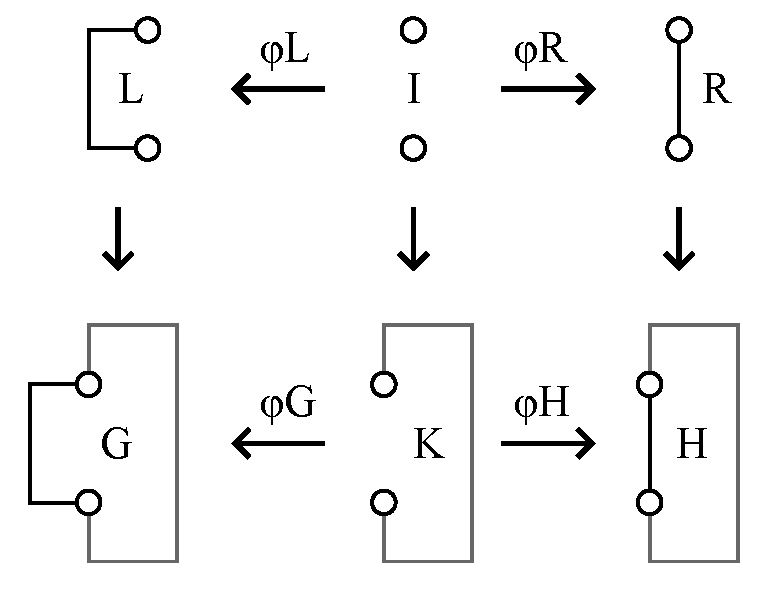
\includegraphics[width=\imgWidth/2]{images/dpo_rule.pdf}
    \caption{Double Pushout Produktionsregel.}
    \label{fig:dpo_rule}
\end{figure}

Die Produktionen im verwendeten \gls{ac:dpo} Ansatz bestehen aus drei Teilen. Einem linken und rechten Graphen (\(L\) und \(R\)), welche jeweils
den Mutter- und Tochtergraphen darstellen, sowie einem Interface-Graphen \(I\), welcher den Einbettungsmechanismus darstellt. Wie in Abbildung
\ref{fig:dpo_rule} zu sehen ist, können diese Graphen mithilfe der Homomorphismen \(\upvarphi L\) und \(\upvarphi R\) untereinander abbilden.

Ein Homomorphismus von Graph \(A\) (mit der Knotenmenge \(V(A)\) und der Kantenmenge \(E(A)\)) zu Graph \(B\) (mit \(V(B)\) und \(E(B)\)) ist eine
Abbildung \(h: A \rightarrow B\), welche alle Knoten in \(V(A)\) auf eine (meist echte) Teilmenge von \(V(B)\) abbildet: \(x, y \in V(A)
\rightarrow h(x), h(y) \in V(B)\). Sind \(x\) und \(y\) in \(A\) adjazent, so müssen \(h(x)\) und \(h(y)\) in \(B\) ebenfalls adjazent sein:
\((x, y) \in E(A) \rightarrow (h(x), h(y)) \in E(B)\). \cite{35_sabidussi}

Ist \(L\) als Teilgraph in einem anderen Graphen \(G\) enthalten, d.h. gibt es einen Homomorphismus \(\upvarphi m: L \rightarrow G\), so kann die entsprechende
Produktion zum Transformieren von \(G\) verwendet werden. Dazu muss \(L\) zunächst aus \(G\) herausgeschnitten werden. Hierfür wird das Interface
benötigt. Dieses beschreibt die Gemeinsamkeiten zwischen der linken und der rechten Seite der Produktion und ermöglicht das problemlose Austauschen
der beiden Seiten miteinander. Wird \(L\) aus \(G\) entfernt, so erhalten wir den sogenannten Klebegraphen \(K\). In diesen können wir nun \(R\)
hineinkleben, um den transformierten Graphen \(H\) zu erhalten. Das Anwenden einer solchen Produktionsregel ist aber auch in die andere Richtung
möglich. Alternativ kann auch zuerst \(R\) aus \(H\) ausgeschnitten und dann dort \(L\) eingeklebt werden, um \(G\) zu produzieren, vorausgesetzt
es gibt einen Homomorphismus \(\upvarphi n: R \rightarrow H\). \cite{7_ehrig_et_al}

\subsubsection{Theorie hinter der Funktionsweise}
Die später aus der Hierarchie abzuleitenden Produktionsregeln werden so angeordnet, dass sich auf der linken Seite ein komplexerer Graph befindet,
als auf der rechten Seiten. Wird die Regel von links nach rechts angwendet, so vereinfacht sie \(G\). Dies bezeichnen wir als \textit{destruktiv}.
Wird sie von rechts nach links angewendet, so macht sie \(H\) komplexer, was wir wiederum als \textit{konstruktiv} berzeichnen.

Wie bereits erwähnt, versuchen wir nach dem Erstellen der einzelnen Graphen Regeln zu finden, die bereits erzeugte Graphen in der Hierarchie
vereinfachen können und entfernen diese dann ggf. aus der Hierarchie. Hier werden die Regeln stets nur destruktiv genutzt, was zunächst unlogisch
erscheint. An diesem Punkt können wir uns die Invertierbarkeit der Produktionen zunutze machen. Wenn wir genug Regeln finden können, um alle Graphen
in der Hierarchie zum leeren Graphen reduzieren zu können, indem wir diese destruktiv verwenden, so können wir im Umkehrschluss genau die gleichen
Regeln konstruktiv benutzen, um aus dem leeren Graphen alle anderen Graphen abzuleiten.

\subsubsection{Ableiten einer Produktionsregel}
Kommen wir nun dazu, wie es möglich ist, solche Regeln automatisch ableiten zu können. Dazu schauen wir uns erneut kurz an, wie eine Produktionsregel
angewandt wird. Wie oben beschrieben, involviert dies zwei Teilschritte. Zunächst wird die eine Seite der Regel aus einem größeren Graphen \(G\)
ausgeschnitten, wodurch dieser zum Klebegraphen \(K\) wird, in welchem nun einige offene Halbkanten enthalten sind. Um \(K\) wieder in einen vollständigen
Graphen \(H\) umwandeln zu können,
müssen all diese Halbkanten anschließend durch Anwenden von entsprechenden Klebeoperationen vervollständig werden. Angenommen, wir haben für den
vorherigen Schritt den Graphen auf der linken Seite der Regel, also \(L\), aus \(G\) ausgeschnitten. Damit der rechte Graph \(R\) die entstandene
Lücke in \(K\) schließen kann, muss dieser exakt die gleichen Halbkanten enthalten, wie \(L\). Besitzt \(R\) weniger Halbkanten, so können einige
der enstandenen Halbkanten in \(K\) nicht vervollständigt werden. Besitzt \(R\) mehr Halbkanten, so würde das Durchführen des Branch Gluings zwischen
\(K\) und \(R\) weitere offene Halbkanten in \(K\) einfügen. Stimmt die Anzahl der Halbkanten in \(L\) und \(R\) überein, aber die Kantenlabel
unterscheiden sich, so kann \(K\) ebenfalls nicht vervollständigt werden. Nur bei hundertprozentiger Übereinstimmung der Halbkanten auf beiden Seiten
der Regel kann diese also problemlos angewandt werden.

Um aus der Hierarchie eine Regel ableiten zu können, müssen wir also jeweils zwei Graphen mit übereinstimmenden Halbkanten finden. Hier können wir uns
den \gls{ac:gbs} zunutze machen, da dieser alle Halbkantenlabel eines Graphen enthält. Besitzen zwei Graphen einen identischen \gls{ac:gbs}, so besitzen
sie zwingend auch die gleichen Halbkanten. Zusätzlich wird durch Abgleichen der Boundary sichergestellt, dass sich an der Planarität des enstehenden
Graphen nach Anwendung einer Produktionsregel nichts ändert. Zwischen den Kanten befinden sich dann nach wie vor die gleichen Drehungen.

Statt einen Graphen \(L\) immer nur mit genau einem anderen Graphen \(R\) zu ersetzen, können wir alternativ auch auf mehrere Graphen \(\{R_1, R_2, \dots\}\)
auf der rechten Seite abbilden, vorausgesetzt diese befinden sich in der Hierarchie. Lassen sich die \gls{ac:gbs} \(\{\partial R_1, \partial R_2, \dots\}\)
zu \(\partial L\) zusammensetzen, so sind ebenfalls alle Bedingungen erfüllt, um die Regel problemlos anwenden zu können. Durch dieses Vorgehen lassen sich
sehr viele weitere Regeln ableiten und das Wachstum der Graph-Hierarchie wird zusätzlich eingeschränkt.

\begin{figure}[t]
    \centering
    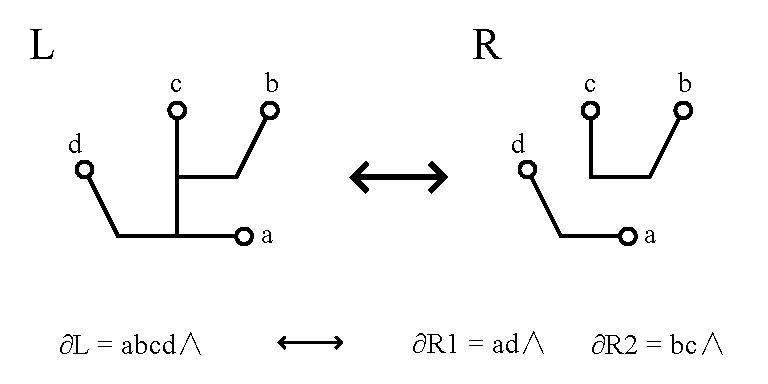
\includegraphics[width=(\imgWidth*3/4)]{images/set_of_graphs.pdf}
    \caption{Ersetzen eines Graphen \(L\) mit mehreren Graphen \(\{R_1,R_2\}\).}
    \label{fig:set_of_graphs}
\end{figure}

Ein Beispiel für eine solche Produktionsregel ist in Abbildung \ref{fig:set_of_graphs} vereinfacht dargestellt. \(\partial L = abcd\wedge\) lässt sich aus
einer Kombination von \(\partial R_1 = ad\wedge\) und \(\partial R_2 = bc\wedge\) bilden. Das Kombinieren von zwei Boundary Strings ist jedoch etwas komplizierter
als das Durchführen einer simplen Konkatenation. Würden wir \(\partial R_1\) und \(\partial R_2\) ohne weitere Anpassungen konkatenieren, so würden wir
einen Boundary String mit zwei positiven Drehungen \(\wedge\) und nicht einer einzigen negativen Drehung \(\vee\) erhalten (z.B. \(a d \wedge b c \vee\)).
Dies würde den Bedingungen für die Planarität widersprechen, da die Differenz zwischen den positiven und negativen Drehungen nun 2 und nicht 1 betragen würde.
Um dieses Problem zu umgehen, wird bei der Kombination zweier \gls{ac:gbs} eine weitere negative Drehung zwischen diesen eingefügt. Nehmen wir an \(A\)
und \(B\) sind Boundary Strings. Die daraus resultierende Kombination hätte dann die Form \(A \vee B\). Dies ist keine willkürliche Anpassung, die
unsere vorher aufgestellten Regeln für einen \gls{ac:gbs} umgeht, sondern eine logische Konsequenz aus diesen. In Abbildung \ref{fig:splicing} ist dies noch einmal
zusätzlich verdeutlicht.

Widmen wir uns nun wieder dem Beispiel in Abbildung \ref{fig:set_of_graphs}. Aufgrund der kreisförmigen Natur eines \gls{ac:gbs} können wir
\(\partial R_1 = ad\wedge\) auch als \(d\wedge a\) und \(\partial R_2 = bc\wedge\) als \(\wedge bc\) darstellen. Werden diese mit einer zusätzlichen
negativen Drehung in der Mitte kombiniert, so erhalten wir \(\partial R_1 \vee \partial R_2 = d\wedge a\vee \wedge bc = d\wedge abc = abcd\wedge = \partial L\).

Mithilfe dieses Wissens können wir nun systematisch eine Vielzahl von Regeln ableiten:
Nach der Erzeugung eines jeden neuen Graphen \(L\) in der Hierarchie betrachten wir stets alle vorher erzeugten Graphen \(R\) und vergleichen die Boundaries
miteinander. Wird dabei eine hunderprozentige Übereinstimmung \(\partial L = \partial R\) gefunden, so kann direkt eine neue Regel abgeleitet werden.
Alternativ könnte \(\partial R\) auch nur ein Teil von \(\partial L\) sein, was einige Teil-Strings hinterlassen würde. Für diese Teil-Strings wird dann
rekursiv nach weiteren Übereinstimmungen gesucht, bis sich \(\partial L \) entweder komplett aus den gefunden Teil-Strings zusammensetzen lässt oder
es keine weiteren Graphen mehr gibt, die noch überprüft werden können. In letzterem Fall kann dann keine Produktionsregel abgeleitet werden.

Betrachten wir erneut das Beispiel in Abbildung \ref{fig:set_of_graphs}. Wir haben einen Graphen \(L\) mit der Boundary \(\partial L = abcd\wedge \) erzeugt.
Beim Iterieren durch die Hierarchie finden wir nun den Graphen \(R_1\) mit \(\partial R_1 = ad\wedge \). \(\partial R_1\) ist als Teil in \(\partial L \)
enthalten, wodurch \(R_1\) also einen Teil von \(L\) ersetzen kann. Übrig bleibt der Teil-String \(bc\). Um diesem einen Graphen zuordnen zu können,
muss zunächst eine positive Drehung \(\wedge \) an diesen angefügt werden. Die zusätzliche Drehung wird dann beim Kombinieren automatisch wieder negiert.
Ein Graph \(R_2\) mit \(\partial R_2 = bc\wedge \) kann anschließend ebenfalls gefunden werden, wodurch alle Teile von \(\partial L\) nun komplett sind. Somit kann
aus den gefundenen eine neue Produktionsregel erstellt und \(L\) aus der Hierarchie entfernt werden, da sich dieser nun nachweislich vereinfachen lässt.

\begin{figure}[t]
    \centering
    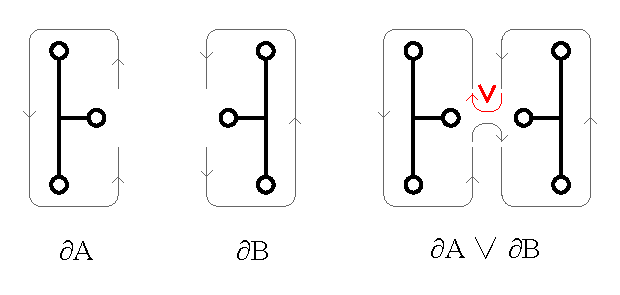
\includegraphics[width=(\imgWidth*3/4)]{images/splicing.pdf}
    \caption{Kombinieren des \gls{ac:gbs} zweier Graphen mit zusätzlicher negativer Drehung.}
    \label{fig:splicing}
\end{figure}

\subsubsection{Starter-Regeln}
Eine Starter-Regel ist eine besondere Produktionsregel, welche den leeren Graphen \(\varnothing\) mit einem vollständigen Graphen ersetzen kann. Davon
kann es theoretisch beliebig viele Regeln geben, jedoch zumindest immer eine. Ohne eine Starter-Regel können keine Graphen aus der Grammatik abgeleitet werden,
da der leere Graph keine Kanten besitzt, auf welche man die Graphen in den anderen Produktionsregeln abbilden könnte. Eine solche Starter-Regel kann durch
das oben beschriebene Vorgehen niemals abgeleitet werden und stellt einen Sonderfall dar. Dieser tritt ein, sobald wir beim Erstellen der Hierarchie
einen vollständigen Graphen \(L\) erzeugen. In diesem Fall wird nicht versucht, \(\partial L\) mit den \gls{ac:gbs} der anderen Graphen in der Hierarchie
abzugleichen. Dies würde ohnehin zu keinem Erfolg führen, da in \(\partial L\) keinerlei Halbkanten enthalten sind. Stattdessen wird \(L\) sofort aus der
Hierarchie entfernt und eine neue Produktionsregel erstellt, welche auf der linken Seite den vollständigen Graphen \(L\) und auf der rechten Seite den
leeren Graphen \(\varnothing\) enthält.

\subsubsection{Eingrenzen des Hierarchie-Wachstums}
Im Optimalfall lassen sich in den ersten paar Generationen der Hierarchie direkt so viele Produktionsregeln ableiten, dass die Hierarchie dadurch vollständig
geleert werden kann. Meist wird dies allerdings nicht eintreffen und die Anzahl der Graphen wächst unkontrollierbar in die Höhe. Nachfolgend werden einige
Optimierungen vorgestellt, um dies etwas weiter einzugrenzen. Leider gibt es selbst dann nach wie vor viele Input-Strukturen, bei denen sich das
Hierarchie-Wachstum nicht ausreichend einschränken lässt. Das Verfahren wird hierdurch dennoch flexibler als auch effizienter.

Eine dieser Optimierungen beläuft sich darauf, ... TODO

% reducing a graph with its descendants (5.4)
% stubs (5.5)
% (5.6)

\section{Erzeugen von Variationen mithilfe der abgeleiteten Regeln}
\subsection{Ableiten eines neuen Winkelgraphen}
Haben wir erfolgreich eine Graph-Grammatik abgeleitet, können wir diese nun verwenden, um daraus neue Winkelgraphen abzuleiten. Dazu wird zunächst eine
Starter-Regel ausgewählt, um eine Grundlage für die weiteren Operationen zu schaffen. Es entsteht ein vollständiger Graph \(G\). Anschließend werden nach
und nach weitere zufällige Produktionsregeln aus der Grammatik ausgewählt und auf den aktuellen Winkelgraphen angewandt. Dabei ist es egal, in welche
Richtung die Regel verwendet wird. Wir können diese sowohl konstruktiv als auch destruktiv benutzen. Um eine Regel anzuwenden, muss der
auszuschneidene Graph \(T\) als Teilgraph in \(G\) enthalten sein. Dies ist der Fall, wenn sich ein Homomorphismus \(m: T \rightarrow G\) finden lässt.
Das Finden eines Homomorphismus zwischen beliebigen Graphen gilt als NP-schweres Problem und
ist somit äußerst kompliziert. \cite{34_cook} Für das Finden von Homomorphismen in planaren Graphen gibt es allerdings effiziente Algorithmen, die in linearer
Zeit zu einem Ergebnis kommen. \cite{8_eppstein} Da wir ausschließlich mit planaren Graphen arbeiten, stellt dies also kein Problem für uns dar. Diesen
Prozess können wir beliebig oft wiederholen und jederzeit abbrechen. Solang zumindest eine Starter-Regel angewandt wurde, erhalten wir in jedem Fall einen
vollständigen Winkelgraphen und somit ein valides Ergebnis für diesen Teilschritt.

\subsection{Festsetzen der Knotenpositionen}
Jetzt gilt es nur noch den eben erzeugten Winkelgraphen in eine Output-Struktur mit festen Knotenpositionen umzuwandeln und gleichzeitig sicherzustellen,
dass diese ohne jegliche Überschneidungen der Kanten dargestellt werden kann. Dazu verwenden wir einen ähnlichen Ansatz wie Bokeloh et al. \cite{4_bokeloh_et_al}
und stellen den Graphen als lineares Gleichungssystem dar, für welches wir anschließend eine Lösung finden. Die einzelnen Gleichungen dieses Systems lassen
sich aus den Kanten des Winkelgraphen ableiten. Die Kanten lassen sich beschreiben durch die Position des Startknotens \(v_0\) und des Endknotens \(v_1\).
Um zu garantieren, dass dabei der Tangentenwinkel der Kante mit dem entsprechenden Winkel \(\theta\) im Kantenlabel übereinstimmt, fügen wir ebenfalls einen
Richtungsvektor \(u\) in die Gleichung mit ein. Dieser kann wie folgt berechnet werden: \(u = [cos(\theta), sin(\theta)]\). Hierbei handelt es sich um einen
Einheitsvektor, der mit einer Kantenlänge \(s\) multipliziert auf die Position von \(v_0\) addiert werden kann, um \(v_1\) zu erhalten. Die gesamte Gleichung
lautet dann: \(v_0 + su = v_1\) bzw. \(v_0 + su - v_1 = 0\). All diese Kantengleichungen können in eine Matrix-Gleichung der Form \(Ax = 0\) gebracht werden,
wobei \(x\) alle Knotenpositionen und Kantenlängen und \(A\) alle Koeffizienten dieser Unbekannten enthält. Durch das Berechnen des Kerns der Matrix \(A\)
lassen sich anschließend mögliche Lösungen für das Gleichungssystem ableiten. Das erstellte Gleichungssystem wird hierbei stets unterbestimmt sein, da es
mehr Unbekannte als Gleichungen gibt. Daraus ergibt sich wiederum, dass es immer entweder keine oder unendlich viele Lösungen geben wird. Wird eine Lösung
gefunden, so enthält diese einige freie Variablen. Somit finden wir statt einer konkreten Lösung immer nur einen Raum an möglichen Lösungen. Diesen Raum
nennen wir Basis des Kerns der Matrix. Durch Festlegen von beliebigen Werten für die freien Variablen können wir daraus nun konkrete Lösungen für das Gleichungssystem
entnehmen. % Abschnitt formaler definieren, Teil zu "Basis des Kerns" überarbeiten

Leider bedeutet das Finden einer Lösung für das Gleichungssystem nicht unbedingt, dass wir nun auch eine valide Darstellung für die Output-Struktur
gefunden haben. Die gefundene Lösung könnte eventuell negative Werte für die Kantenlängen enthalten, welche nicht dargestellt werden können. Um dies zu umgehen,
müssen wir die vorgeschlagenen Lösungen also stets auf ungültige Werte überprüfen und ggf. eine neue Lösung generieren. Neben dem Überprüfen auf negative
Kantenlängen könnten wir hier außerdem weitere durch den Endnutzer angegebene Kriterien überprüfen und so z.B. alle Kantenlängen auf einen bestimmten Wertebereich
beschränken.

% Eingehen auf Optimierung durch inkrementelles Vorgehen (6.2)

% TODO:
% - Referenzieren von Bildern
% - Hinzufügen von Quellen
% @author Benjamin Schröder
%
\chapter{Implementierung}
Im folgenden Kapitel betrachten wir die praktische Implementierung der zuvor vorgestellten Konzepte. Dazu werden zunächst
einige spezifische Anforderungen an die zu entwickelnde Software aufgelistet. Anschließend wird darauf eingegangen, wie
diese Anforderungen dann umgesetzt werden sollen, indem die verwendeten Technologien und Entwurfsmuster vorgestellt werden.

\section{Anforderungen an die Software}
\subsection{Funktionale Anforderungen}
Die funktionalen Anforderungen beschreiben, \textit{was} umgesetzt werden soll, also welche konkreten Funktionen von der Software
bereitgestellt werden sollen. Diese lauten wie folgt:

\begin{itemize}
    \item es sollen beliebige polygonale 2D-Strukturen als Input eingelesen werden können
    \item es sollen einige Beispielstrukturen als Input zur Verfügung gestellt werden, zwischen denen der Nutzer auswählen kann
    \item mithilfe einer polygonalen Struktur als Input sollen automatisch ähnliche Strukturen generiert werden können:
    \begin{itemize}
        \item aus einer eingelesenen Input-Struktur sollen automatisch Regeln für eine Graph-Grammatik abgeleitet werden können
        \item aus einer gegebenen Graph-Grammatik sollen verschiedene Graphen abgeleitet werden können
        \item aus einem solchen Graphen soll dann eine planare Output-Struktur mit fester Geometrie (also festen Knotenpositionen) erzeugt werden können
    \end{itemize}
    \item es soll eine Benutzeroberfläche geben, in welcher der Nutzer Parameter für die Generierung einstellen sowie verschiedene Inputstrukturen auswählen können soll
    \item sowohl die Input-Strukturen, die daraus erzeugt Grammatik und die generierten Variationen sollen visualisiert werden können
\end{itemize}

\subsection{Nicht-funktionale Anforderungen}
Die nicht-funktionalen Anforderungen beschreiben, \textit{wie} die oben aufgelisteten Funktionen umgesetzt werden sollen, also
welche Qualitätskriterien dabei eingehalten werden sollen. Diese lauten wie folgt:

\begin{itemize}
    \item die Anwendung soll auf Windows ausführbar sein
    \item die Nutzeroberfläche soll einfach und übersichtlich gehalten werden
    \item die implementierten Algorithmen sollen sich deterministisch verhalten und durch einen Seed reproduzierbar sein
    \item alle wichtigen Komponenten sollen durch Tests abgedeckt sein
    \item alle nicht-trivialen Bestandteile des Codes sollen mit Kommentaren versehen werden
    % TODO: Anforderungen an Input-Größe, Zeitverhalten, und Architektur (Kopplung, etc.)
\end{itemize}

\section{Verwendete Technologien und Bibliotheken}
Der gesamte Code ist in Java 16 geschrieben. Die grafische Benutzeroberfläche wird mithilfe des Java GUI-Toolkits Swing umgesetzt,
welches Bestandteil der Java-Runtime ist und viele Bibliotheken zum Erstellen von simplen Nutzeroberflächen bereitstellt. Die
entwickelte Software wird hierbei als Teil eines größeren \gls{ac:pcg}-Projekts von Prof. Dr. Philipp Jenke umgesetzt, in welchem
sich viele weitere Studenten-Projekte, sowie Implementierungen von weiteren Algorithmen und Datenstrukturen im Bereich der prozeduralen
Generierung befinden. Die grundsätzlichen von uns verwendeten Datenstrukturen und Algorithmen werden jedoch allesamt selbst implementiert
und wir bedienen uns lediglich einiger Helfer-Funktionen, z.B. für das Einlesen von Dateien oder dem Loggen des Programmablaufs.

\section{Architektur}
% TODO

\section{Datenstrukturen}
Grundsätzlich werden drei verschiedene Datenstrukturen implementiert, welche nachfolgend vorgestellt werden.

\subsection{PolygonMesh}
%\lstinline{code}
Die \codeword{PolygonMesh}-Klasse repräsentiert die in \autoref{chap:input} vorgestellte polygonale Struktur, die der Algorithmus
als Input bekommt und als Output erzeugt. Jedes \codeword{PolygonMesh}-Objekt verwaltet eine Liste von Knoten (Klasse \codeword{Vertex}),
eine Liste von Kanten (Klasse \codeword{Edge}) und eine Liste von Polygonen (Klasse \codeword{Polygon}). Diese werden alle auf der
obersten Ebene (also in der \codeword{PolygonMesh}-Klasse) verwaltet, um das Vorhandensein von Duplikaten zu verhindern. Da sich
mehrere Polygone die gleichen Kanten, und mehrere Kanten die gleichen Knoten teilen können, kann es sonst vorkommen, dass diese mehrfach
in der Datenstruktur gespeichert werden. Durch die Verwaltung aller Instanzen der anderen Klassen in \codeword{PolygonMesh} selbst wird
dies verhindert.

Ein \codeword{Vertex} besitzt lediglich nur ein einziges Feld: eine zweidimensionale Knotenposition und kann dadurch vollständig
beschrieben werden. Eine \codeword{Edge} wird durch zwei verschiedene Knoten definiert. Für diese wird jeweils nur ein Index gespeichert,
über welchen das eigentliche \codeword{Vertex}-Objekt in der Liste in \codeword{PolygonMesh} referenziert werden kann. Die Felder in
\codeword{Polygon} werden ähnlich umgesetzt: auch hier werden wieder nur Indexe für die untergeordneten Objekte gespeichert. Jedes
\codeword{Polygon} besitzt dabei eine Liste von Kanten- als auch Knoten-Indexen. Außerdem enthält jedes \codeword{Polygon} ein Feld
für eine Farbe, welche später genutzt wird, um dieses in der grafischen Darstellung einzufärben.

Neben der Verwaltung der eigentlichen Datenstruktur stellt die \codeword{PolygonMesh}-Klasse außerdem Funktionalität zum Serialisieren
und Deserialisieren der Objekte bereit. Ein \codeword{PolygonMesh}-Objekt kann in eine \codeword{.mesh}-Datei umgewandelt werden und umgekehrt
kann ein neues \codeword{PolygonMesh}-Objekt durch das Einlesen einer \codeword{.mesh}-Datei initialisiert werden. So können wir neue
\codeword{PolygonMesh}-Objekte zur Laufzeit erzeugen. In einer \codeword{.mesh}-Datei werden alle Knotenpositionen, die Knoten-Indexe der einzelnen
Polygone, sowie die Polygonfarben als Plain-Text abgespeichert. Dies ermöglicht das einfache Erstellen von neuen Polygon-Strukturen, die
dann dem Nutzer als Input für den Algorithmus bereitgestellt werden.

\subsection{AngleGraph}

\subsection{GraphGrammar}

\section{Algorithmen}

\section{Ablauf}

% @author Benjamin Schröder
%
\chapter{Auswertung}
\label{chap:auswertung}
Werten wir die vorgestellte Implementierung nun aus. Dazu überprüfen wir zunächst die anfangs vorgestellten Anforderungen an die gesamte
Software und diskutieren anschließend, wie erfolgreich dabei das eigentliche Verfahren umgesetzt wurde. Dazu werden einige
Beispieldurchläufe mit verschiedenen Parameter-Werten betrachtet.

\section{Überprüfen der Anforderungen}
\subsection{Funktionale Anforderungen}
\subsubsection{Funktionale Anforderung 1}
\textit{Es sollen beliebige polygonale 2D-Strukturen als Input eingelesen werden können.} Diese Anforderung wird
durch die entwickelte \code{PolygonMesh} Datenstruktur realisiert. In dieser können beliebige Polygone in eine größere zusammenhängende
Struktur gebracht werden. Diese Datenstruktur kann von der \code{GrammarBuilder} Klasse als Input entgegengenommen werden, was die
Grundlage für das Durchführen aller weiteren Teilschritte des Verfahrens darstellt.

\subsubsection{Funktionale Anforderung 2}
\textit{Es sollen einige Beispielstrukturen als Input zur Verfügung gestellt werden, zwischen denen der Nutzer auswählen kann.}
Dies wird durch die vorgestellte \code{InputScene} realisiert. Hier kann der Benutzer ein Dropdown-Menü öffnen und erhält eine Liste an
möglichen Beispielstrukturen, die alle vom \code{InversePcgController} in ein \code{PolygonMesh} Objekt umgewandelt werden können.
Beispielstrukturen können ohne viel Aufwand und ohne Anpassung des Codes entfernt, hinzugefügt oder ausgetauscht werden, da diese in
separaten \code{.mesh}-Dateien gespeichert werden und dynamisch zur Laufzeit eingelesen werden können.

\subsubsection{Funktionale Anforderung 3}
\textit{Es sollen automatisch zum Input lokal ähnliche Strukturen generiert werden können.} Die Theorie hinter dem implementierten Verfahren beruht
vollständig auf den in \autoref{chap:konzept} vorgestellten Konzepten und erzeugt den Output nach dem dort beschriebenen Vorgehen. Ist das Verfahren
erfolgreich durchgelaufen, so lässt sich jeder Teil der dadurch erzeugten Outputstruktur im Input wiederfinden und die erzeugte Strukture ist somit
lokal ähnlich zum Input. In vielen Fällen kann das Verfahren aufgrund von Defiziten in der \code{MeshSolver} Komponente jedoch nicht erfolgreich durchlaufen,
wodurch diese Anforderung nicht immer vollständig erfüllt werden kann.

\textit{a) Aus einer eingelesenen Inputstruktur sollen automatisch Regeln für eine Graphgrammatik abgeleitet werden können.} Diese Anforderung wird
durch die Klasse \code{GrammarBuilder} realisiert, welche ein gegebenes \code{PolygonMesh} Objekt in eine \code{GraphGrammar} umwandeln kann.

\textit{b) Aus einer gegebenen Graphgrammatik sollen verschiedene Graphen abgeleitet werden können.} Hierfür ist die \code{GraphBuilder} Klasse zuständig.
Der dort entwickelte Algorithmus nimmt ein \code{GraphGrammar} Objekt entgegen und erzeugt daraus ein neues \code{AngleGraph} Objekt.

\textit{c) Aus einem solchen Graphen soll dann eine planare Outputstruktur mit fester Geometrie (also festen Knotenpositionen) erzeugt werden können.}
Dies wird vom \code{MeshSolver} übernommen, welcher ein \code{AngleGraph} Objekt in ein \code{PolygonMesh} Objekt umwandeln kann. Hier gibt es allerdings
das Problem, dass in vielen Fällen keine valide Lösung für die Outputstruktur gefunden werden kann. Bei der Verarbeitung etwas größerer Winkelgraphen
entstehen beim Lösen des entstandenen Gleichungssystems so viele freie Variablen, dass es eine ziemlich große Wahrscheinlichkeit gibt, dass zumindest
eine dieser Variablen zum Erzeugen von ungültigen Werten für eine der anderen unbekannten Variablen führt. Dies versuchen wir zu umgehen, indem
dieser Vorgang bis zu \code{maxTries} Mal wiederholt wird, in der Hoffnung, dass die jeweils nächste zufällige Lösung gültig sein wird. Da jedes Mal
jedoch alle Variablen erneut generiert werden, ist die Fehlerwahrscheinlichkeit dabei so hoch, dass in den meisten Fällen auch nach etlichen Versuchen
keine valide Lösung generiert werden kann. In diesem Fall visualisieren wir trotzdem die zuletzt erzeugte Struktur, jedoch wird diese nicht vollständig
zum Input lokal ähnlich sein.

\subsubsection{Funktionale Anforderung 4}
\textit{Es soll eine grafische Benutzeroberfläche geben, in welcher der Nutzer Parameter für die Generierung einstellen, sowie zwischen
den verschiedenen Inputstrukturen auswählen können soll.} Dies wird durch die Klasse \code{InversePcgApplication} realisiert. In den drei darin
implementierten Szenen kann der Nutzer alle wichtigen Einstellungen vornehmen. In der \code{InputScene} kann der Seed für den Zufallsgenerator festgelegt
und eine Inputstruktur ausgewählt werden. In der \code{GrammarScene} kann die Anzahl an Generation in der Graph-Hierarchie festgelegt werden. In der
\code{OutputScene} können alle weiteren in \autoref{chap:datenmodell} vorgestellten Parameter eingestellt werden.

\subsubsection{Funktionale Anforderung 5}
\textit{Sowohl die Inputstrukturen, die daraus erzeugt Grammatik und die generierten Variationen sollen visualisiert werden können.} Die Visualisierung
der hier genannten Datenstrukturen wird ebenfalls durch die \code{InversePcgApplication} übernommen. In der \code{InputScene} wird die ausgewählte
Inputstruktur dargestellt, die \code{GrammarScene} übernimmt das Darstellen der daraus erzeugten Grammatik, und die \code{OutputScene} wird zum
Visualisieren der verschiedenen erzeugten Variationen benutzt.

\subsection{Nichtfunktionale Anforderungen}
\subsubsection{Nichtfunktionale Anforderung 1}
\textit{Die Anwendung soll auf Windows ausführbar sein.} Der gesamte Code wurde auf einem Windows 11 PC und einem Laptop mit Windows 10 implementiert
und getestet. Bei der Ausführung der Anwendung auf beiden Geräten gibt es keine Probleme. Die Anforderung wurde also erfüllt.

\subsubsection{Nichtfunktionale Anforderung 2}
\textit{Die Nutzeroberfläche soll einfach und übersichtlich gehalten werden.} Die implementierte Benutzeroberfläche wurde sehr simpel gestaltet und
stellt nur die wichtigsten Funktionen bereit. Es gibt lediglich drei verschiedene Szenen, welche jeweils nur aus einem Viewport und einer kurzen
Reihe an Einstellungsmöglichkeiten, sowie einem Knopf zum Senden eines Befehls an die Steuerungskomponente bestehen. Alles wird in einem Fenster
dargestellt, es gibt keine Pop-ups und mit der Ausnahme des Dropdown-Menüs zum Auswählen der Inputstruktur auch keine aufklappbaren Komponenten mit
versteckter Komplexität. Da die Anwendung vollständig mit Swing und AWT umgesetzt wurde, ist das Design der verwendeten GUI-Komponenten selbst ebenfalls
sehr simpel gehalten.

\subsubsection{Nichtfunktionale Anforderung 3}
\textit{Die implementierten Algorithmen sollen sich deterministisch verhalten und alle Ergebnisse sollen reproduzierbar sein.} Auch diese Anforderung
wird erfüllt. Alle Algorithmen, bei denen das Erzeugen von Zufallszahlen eine Rolle spielt, erhalten die Zufallszahlen von ein und demselben
Zufallszahlengenerator, der von der Steuerungskomponente verwaltet wird. Dieser wird stets mit einem vom Benutzer festgelegten Seed initialisiert und
erzeugt bei gleichem Seed stets die gleichen zufälligen Zahlen. Werden vom Nutzer nach Start der Anwendung die exakt gleichen Aktionen immer und immer
wiederholt, so sind die erzeugten Ergebnisse ebenfalls immer und immer wieder identisch.

\subsubsection{Nichtfunktionale Anforderung 4}
\textit{Die Software soll modular aufgebaut sein, wobei die Module selbst eine hohe Kohäsion vorweisen und untereinander schwach gekoppelt sein sollen.}
Wie in \autoref{chap:architektur} ausführlich erklärt wurde, besteht die entwickelte Software aus vielen verschiedenen in sich logisch gekapselten Komponenten.
Aufgrund des gewählten \gls{ac:mvc}-Entwurfsmusters sind die drei Hauptkomponenten Ansicht, Datenmodell und Steuerung lose untereinander gekoppelt und können
größtenteils unabhängig voneinander existieren. \cite{48_bucanek} Es werden einheitliche Schnittstellen geboten oder die Informationen werden über das Beobachter-Muster
zwischen den Komponenten ausgetauscht. In beiden Fällen wäre ein Austauschen der einzelnen Komponenten ledglich mit sehr geringem Aufwand verbunden. Die
Kohäsion innerhalb der einzelnen Module ist hoch, da diese jeweils einen klar definierten Aufgabenbereich haben und die gesamte darin umgesetzte Funktionalität
nur zum Umsetzen der entsprechenden Aufgabe des Moduls genutzt wird. Funktionalität, die sich von mehreren Komponenten geteilt wird, wurde in eine separate
Klasse \code{Utils} ausgelagert. Die Komponenten mit der niedrigsten Kohäsion sind die Klassen \code{PolygonMesh} und \code{AngleGraph}, da diese neben dem
Definieren der entsprechenden Datenstruktur auch komplexere Funktionalität für die Transformation dieser Datenstruktur enthalten. Diese Funktionalität
hätte jeweils eventuell auch in eine separate Klasse ausgelagert werden können.

\subsubsection{Nichtfunktionale Anforderung 5}
\textit{Alle wichtigen Komponenten sollen durch Tests abgedeckt sein.} Diese Anforderung wurde größtenteils umgesetzt. Es gibt separate Testklassen für
die drei implementierten Algorithmus-Klassen \code{GrammarBuilder}, \code{GraphBuilder} und \code{MeshSolver}. In diesen wird jeweils der gesamte Ablauf
des entsprechenden implementierten Teilschritts getestet, indem die erhaltenen Endergebnisse überprüft werden. Außerdem befinden sich dort Tests für
viele, aber nicht alle, Teilfunktionen, die dabei genutzt werden. Auch für die Datenstrukturen gibt es Tests, allerdings nur für die Klassen \code{AngleGraph}
und \code{PolygonMesh}, da diese Funktionalität für komplexere Transformationen der entsprechenden Datenstrukturen enthalten.

\subsubsection{Nichtfunktionale Anforderung 6}
\textit{Der Code soll verständlich sein und alle nicht-trivialen Bestandteile des Codes sollen mit Kommentaren versehen werden.} Jede von uns selbst
implementierte und nicht von anderen Klassen geerbte Methode wurde mit Javadoc-Kommentaren versehen, die die genaue Funktionsweise, die involvierten
Paramater und den Rückgabewert der Methode erklären. Komplexere Methoden wurden außerdem intern mit weiteren Kommentaren versehen, wenn die einzelnen
Teilschritte als nicht-trivial erachtet wurden. Die Benennung der verschiedenen Klassen, Methoden und Variablen wurde so gewählt, dass diese so präzise
wie möglich den entsprechenden Zweck beschreiben. Generell wurde der Code auf Basis der in \cite{49_java_conventions} vorgestellten Konventionen erstellt.
Damit gilt diese Anforderung als erfüllt.

\section{Beispieldurchläufe}
Nachfolgend werden einige der erhaltenen Ergebnisse präsentiert, welche mithilfe von verschiedenen Parameter-Konfigurationen erzeugt wurden. Zunächst
zeigen wir einige erfolgreiche Ergebnisse. Es werden jeweils die verwendete Inputstruktur, die daraus erzeugte Grammatik, sowie die letztendliche Outputstruktur
dargestellt. Die Grammatik kann in den meisten Fällen aufgrund der großen Anzahl an Regeln nicht vollständig dargestellt werden und es wird jeweils nur ein
Ausschnitt an Regeln gezeigt. Außerdem werden die verwendeten Parameter-Konfigurationen für jedes Beispiel gezeigt.

\subsection{Erfolgreiche Durchläufe}

Für den in Abbildung \ref{fig:house_success} dargestellten Durchlauf verwendete Parameter: \code{seed = 23456}, \code{maxGeneration = 6}, \code{iterations = 5},
\code{maxTries = 100}, \code{minRandVal = 10}, \code{maxRandVal = 100}. Die Ergebnisse entsprechen den Erwartungen.
\begin{figure}[H]
    \centering
    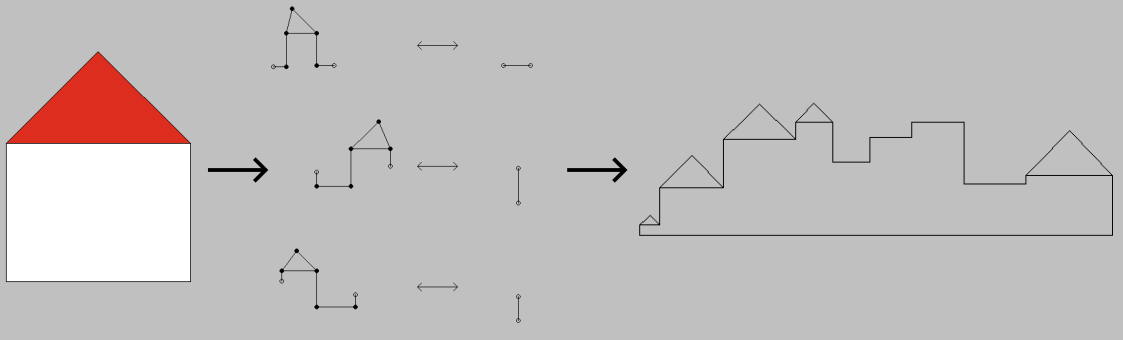
\includegraphics[width=\textwidth]{images/house_success.png}
    \caption{Erfolgreicher Durchlauf mit Input-Datei \code{house.mesh}.}
    \label{fig:house_success}
\end{figure}

Für den in Abbildung \ref{fig:square_double_success} dargestellten Durchlauf verwendete Parameter: \code{seed = 77}, \code{maxGeneration = 3}, \code{iterations = 7},
\code{maxTries = 100}, \code{minRandVal = 10}, \code{maxRandVal = 100}. Die Ergebnisse entsprechen den Erwartungen.
\begin{figure}[H]
    \centering
    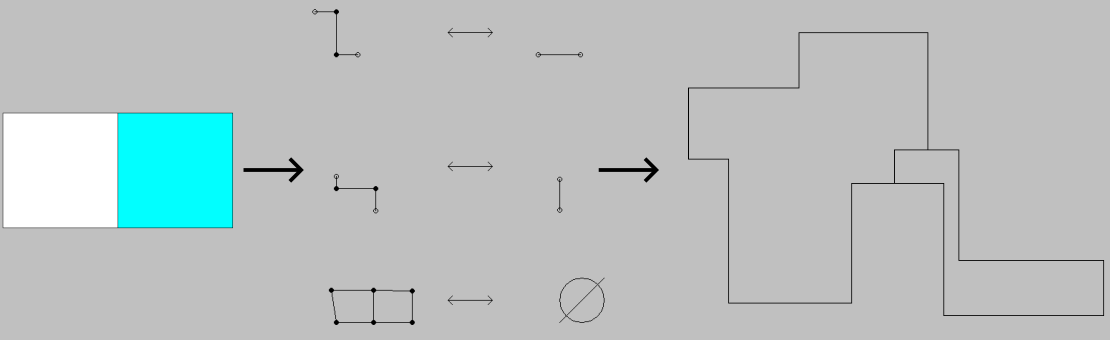
\includegraphics[width=\textwidth]{images/square_double_success.png}
    \caption{Erfolgreicher Durchlauf mit Input-Datei \code{square\_double.mesh}.}
    \label{fig:square_double_success}
\end{figure}

Für den in Abbildung \ref{fig:square_success} dargestellten Durchlauf verwendete Parameter: \code{seed = 5555}, \code{maxGeneration = 3}, \code{iterations = 5},
\code{maxTries = 100}, \code{minRandVal = 10}, \code{maxRandVal = 10}. Die Ergebnisse entsprechen den Erwartungen. Durch das Limitieren der Zufallszahlen auf nur
exakt einen Wert enthält der Output sehr viele Kanten mit der gleichen Kantenlänge und nimmt somit eine regelmäßige Form an. Es wirkt, als wäre der Output auf
Basis eines Gitters modelliert worden.
\begin{figure}[H]
    \centering
    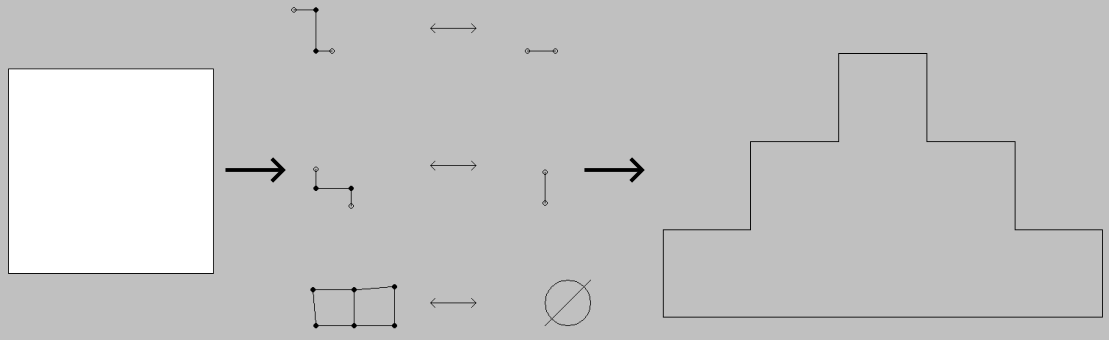
\includegraphics[width=\textwidth]{images/square_success.png}
    \caption{Erfolgreicher Durchlauf mit Input-Datei \code{square.mesh}.}
    \label{fig:square_success}
\end{figure}

Für den in Abbildung \ref{fig:rhombus_success} dargestellten Durchlauf verwendete Parameter: \code{seed = 123}, \code{maxGeneration = 3}, \code{iterations = 10},
\code{maxTries = 100}, \code{minRandVal = 10}, \code{maxRandVal = 70}. Die Ergebnisse entsprechen den Erwartungen.
\begin{figure}[H]
    \centering
    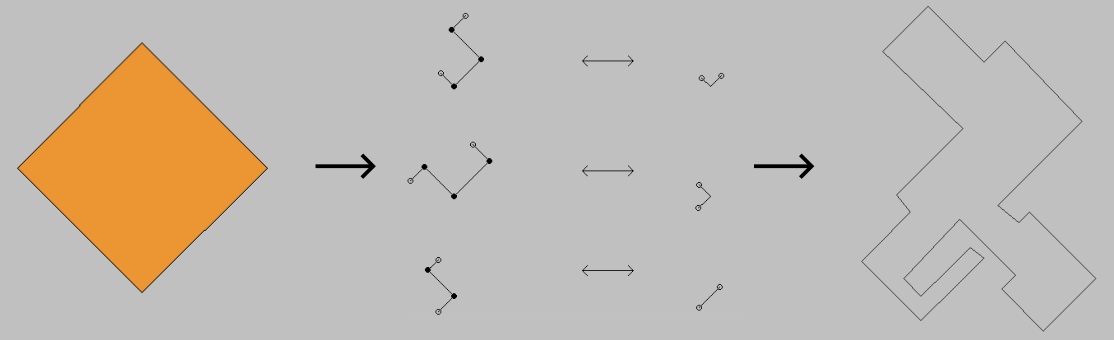
\includegraphics[width=\textwidth]{images/rhombus_success.png}
    \caption{Erfolgreicher Durchlauf mit Input-Datei \code{rhombus.mesh}.}
    \label{fig:rhombus_success}
\end{figure}

\subsection{Fehlerhafte Durchläufe}

Für den in Abbildung \ref{fig:house_fail} dargestellten Durchlauf verwendete Parameter: \code{seed = 337}, \code{maxGeneration = 7}, \code{iterations = 7},
\code{maxTries = 100}, \code{minRandVal = 10}, \code{maxRandVal = 100}. Die Ergebnisse entsprechen nicht den Erwartungen. Alle dargestellten Kantenwinkel
lassen sich zwar im Input wiederfinden und es wirkt so, als wäre die erzeugte Outputstruktur zumindest lokal ähnlich zum Input. Das Ergebnis ist jedoch
trotzdem fehlerhaft, da sich einige der Kanten überschneiden.
\begin{figure}[H]
    \centering
    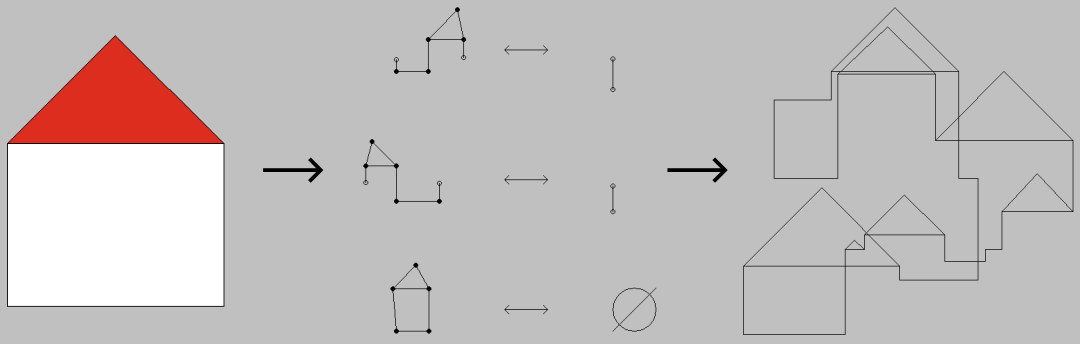
\includegraphics[width=\textwidth]{images/house_fail.png}
    \caption{Fehlerhafter Durchlauf mit Input-Datei \code{house.mesh}.}
    \label{fig:house_fail}
\end{figure}

Für den in Abbildung \ref{fig:octagon_fail} dargestellten Durchlauf verwendete Parameter: \code{seed = 445}, \code{maxGeneration = 2}, \code{iterations = 7},
\code{maxTries = 10}, \code{minRandVal = 10}, \code{maxRandVal = 100}. Diesmal ist der dargestellte Output planar, jedoch liegt hier keine lokale Ähnlichkeit
vor. Die Kantenwinkel stimmen zwar alle mit den Kantenwinkeln im Input überein, jedoch unterscheidet sich die Topologie der beiden Strukturen an einigen Stellen.
Einige der Knoten in der Outputstruktur (an den ``Spitzen'') lassen sich nicht im Input wiederfinden.
\begin{figure}[H]
    \centering
    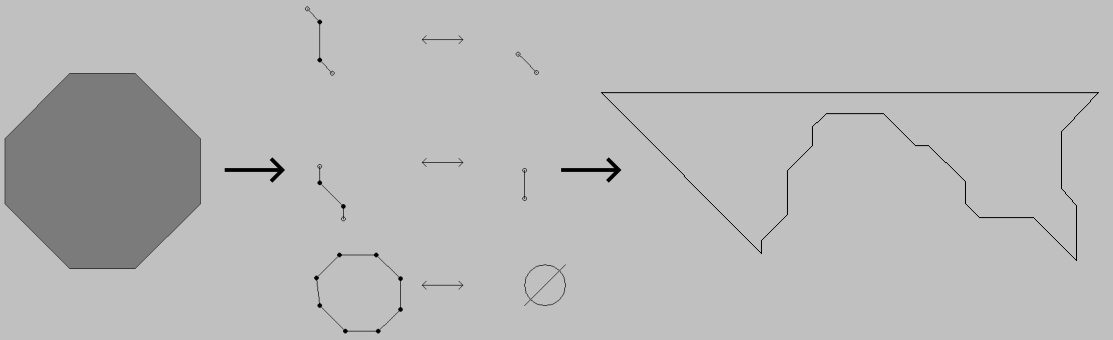
\includegraphics[width=\textwidth]{images/octagon_fail.png}
    \caption{Fehlerhafter Durchlauf mit Input-Datei \code{octagon.mesh}.}
    \label{fig:octagon_fail}
\end{figure}

Für den in Abbildung \ref{fig:triangle_fail} dargestellten Durchlauf verwendete Parameter: \code{seed = 23456}, \code{maxGeneration = 30}, \code{iterations = 3},
\code{maxTries = 100}, \code{minRandVal = 10}, \code{maxRandVal = 100}. Der Output entspricht den geforderten Eigenschaften, ist sowohl zum Input lokal
ähnlich als auch planar und somit nicht fehlerhaft. Trotzdem ist das Ergebnis unbrauchbar, da sich der Output kaum vom Input unterscheidet. Der Output
besitzt zwar andere Kantenlängen, ist strukturell allerdings exakt gleich aufgebaut. Trotz der hohen Anzahl an zugelassenen Generationen konnte das Verfahren
lediglich nur eine einzige Starter-Regel für die Grammatik ableiten (beide dargestellten Starter-Regeln sind identisch). Aus dieser Grammatik kann keine
hohe Vielfalt an Ergebnissen erzeugt werden.
\begin{figure}[H]  
    \centering  
    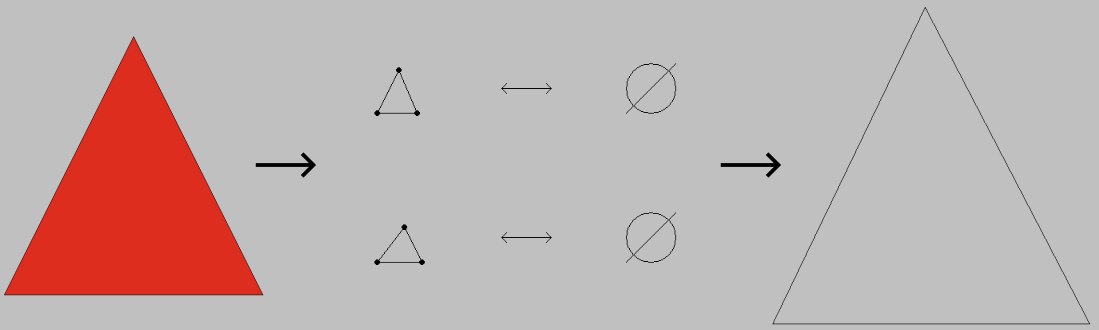
\includegraphics[width=\textwidth]{images/triangle_fail.png}
    \caption{Ungenügender Durchlauf mit Input-Datei \code{triangle.mesh}.}
    \label{fig:triangle_fail}
\end{figure}

\section{Auswertung der Ergebnisse}
Allgemein sind die Ergebnisse durchaus zufriedenstellend. Die erzeugten Strukturen erfüllen zwar in vielen Fällen nicht die Anforderungen an die lokale
Ähnlichkeit und können auch oft nicht ohne Überschneidungen einiger der Kanten dargestellt werden, jedoch wird durch die von uns implementierte Software
klar demonstriert, dass dieses Verfahren grundsätzlich funktioniert. Auch wenn es dabei noch viele Probleme gibt, die behoben werden müssen um dieses
Verfahren wirklich in der Praxis einsetzen zu können, erfüllt die entwickelte Anwendung voll und ganz ihren Zweck als Prototyp.

% @author Benjamin Schröder
%
\chapter{Fazit} % Auswerten der gesamten Arbeit
Abschließend soll diese Arbeit kurz reflektiert werden. Dazu fassen wir die gewonnenen Erkenntnisse zusammen und geben
anschließend einen Ausblick auf mögliche Verbesserungen und Erweiterungsmöglichkeiten des vorgestellten Ansatzes und
seiner Umsetzung.

\section{Zusammenfassung}

\section{Verbesserungsansätze und Erweiterungsmöglichkeiten}


%\bibliographystyle{plain}
\bibliographystyle{dinat}
\bibliography{literature}

% Appendix
\appendix
% !TEX root = ../thesis.tex
% appendix example chapter
% @author Thomas Lehmann
%

\chapter{Anhang}

\section{Verwendete Hilfsmittel}
In der Tabelle \ref{tab:tooling} sind die im Rahmen der Bearbeitung des Themas der \IthesisKindDE~verwendeten Werkzeuge und Hilfsmittel aufgelistet.

\begin{table}[h!]
\caption{Verwendete Hilfsmittel und Werkzeuge}
\begin{tabular}{|l|l|}
\hline 
\rowcolor{lightgray} Tool & Verwendung \\
\hline
ChatGPT & Künstliche Intelligenz verwendet als Hilfe bei der Literaturrecherche \\
\hline
Inkscape & Vektorgrafik-Software verwendet zur Erstellung von Abbildungen \\
\hline
draw.io & UML-Modellierungs-Software verwendet für den Architekturentwurf \\
\hline
\end{tabular}
\label{tab:tooling}
\end{table}


\IGlossary

\Istatement

\end{document}

% compile using the following commands:
%
% pdflatex thesis.tex
% bibtex thesis
% makeglossaries thesis
% pdflatex thesis.tex
% pdflatex thesis.tex
